\section{Hardware}
\label{h_hardware}

\subsection{Requerimientos}
\label{h_requerimientos}

Nuestro proyecto...


\subsection{Ideas de implementaci\'on}
\label{h_ideas}

Evaluamos distintos factores para la elecci\'on de cada dispositivo o m\'odulo presente en el robot.
Desde la forma de desplazamiento hasta el m\'etodo de sensado, pasando por el controlador, captura
de im\'agenes y m\'etodo de recolecci\'on de residuos.
Estos son los factores que explicamos y detallamos en este apartado.

\subsubsection{Locomoci\'on}
\label{h_ideas_locomocion}

Un robot m\'ovil se caracteriza por su capacidad de desplazarse por el entorno.
Es por esto que la locomoci\'on es un factor importante que tuvimos que resolver.

La forma que usar\'ia el robot para desplazarse, si ser\'ia mediante ruedas, orugas o patas nos
iba a determinar las necesidades de control, equilibrio, capacidad de coordinaci\'on, velocidad
y hasta la autonom\'ia.

El uso de orugas era una excelente opci\'on como base para soporte del peso y prove\'ia buen
equilibrio, pero la fricci\'on de las mismas generaba una posible falta de precisi\'on que nos
pod\'ia traer problemas para la detecci\'on de la cantidad de giro o desplazamiento y por ende,
una incorrecta localizaci\'on en el terreno.
Por otra parte, la coordinaci\'on de las patas y el equilibrio del cuerpo implicaba una
complejidad que escapaba el alcance del proyecto.

El uso de dos ruedas de tracci\'on y con al menos una tercer rueda de tipo castor para proveer
equilibrio fue nuestra elecci\'on de dise\~no.

En la secci\'on \ref{h_actuadores} explicamos detalladamente la elecci\'on de los actuadores
para esta tarea.

\subsubsection{Sensado del entorno}
\label{h_ideas_sensado}

El sensado del ambiente englobaba varios puntos que deb\'iamos tener en cuenta a la hora de elegir
la cantidad, forma, rango, m\'etodo y costo de los sensores.
En principio los requerimientos eran claros, necesitabamos poder detectar objetos en el ambiente,
evitar obst\'aculos y realizar mediciones internas al robot, como eran el nivel de bater\'ia,
consumo y posici\'on de los motores.

La captura de im\'agenes deb\'ia ser realizada por medio de una c\'amara de video o webcam.
\'Esta prove\'ia de la principal fuente de datos para el proceso de reconocimiento de residuos
explicado en el documento.
Las distintas caracter\'isticas de la c\'amara como su resoluci\'on, refresco, nivel de ruido,
mejoras de la im\'agen y su velocidad de respuesta nos determinar\'ian la elecci\'on de la misma.

La detecci\'on de obst\'aculos implicaba sensores con caracter\'isticas diferentes.
Principalmente necesitabamos sensores de distancia con la apertura necesaria para cubrir lo
mejor posible, el per\'imetro del robot, otorgando un rango de detecci\'on lo suficientemente olgado
que permitiera una adecuada velocidad de respuesta al controlador principal para poder
evitar objetos desconocidos o marcados como obst\'aculos.

Entre los distintos tipos de sensores de distancia estaban los de ultrasonido, tel\'emetros infrarrojos
y scanners l\'aser.
Los sensores de distancia por ultrasonido tienen un rango aproximado entre 2 cent\'imetros y 4 metros
en la zona de detecci\'on y un \'angulo de apertura variable seg\'un la distancia al objetivo.
El tiempo de espera que debemos tener entre disparo y disparo del sensor por posibles rebotes del pulso
de sonido es relativamente elevado, lo que no lo hace el m\'as adecuado para colocarlo a lo largo del
per\'imetro del robot.
En contraparte los tel\'emetros infrarrojos no poseen esta limitaci\'on en cuanto a los rebotes.
Pero los rangos efectivos de detecci\'on de objetos no cubrian completamente nuestras necesidades.

Debido a las caracter\'isticas de cada sensor decidimos combinarlos para aprovechar los beneficios y
suplir las falencias de un tipo con otro el tipo.
Un anillo de 8 tel\'emetros distribuidos de forma tal que haya una mayor resoluci\'on en la zona frontal
del robot contra la zona trasera y lateral y un \'unico sensor de distancia por ultrasonido al frente
para captar objetos a mayor distancia fue nuestra elecci\'on.

El uso de un scanner l\'aser hubiera sido ideal para un an\'alisis topogr\'afico del terreno, aunque \'esto
no era un requerimiento de nuestro proyecto y el elevado costo se escapaba de nuestra escala.

La detecci\'on de una l\'inea en el suelo la resolvimos mediante el uso de sensores \'opticos reflectivos
apuntando hacia el piso de manera tal que permitieran diferenciar entre distintos niveles de reflexi\'on
y por ende, diferenciar una l\'inea del piso.

En la secci\'on \ref{h_sensado} explicamos con m\'as detalle cada uno de los sensores elegidos.

\subsubsection{Controlador}
\label{h_ideas_controlador}

Ten\'iamos especificaciones que nos generaban la necesidad de ejercer control sobre los distinos dispositivos
presentes en el robot, ya sea para configurar o obtener la informaci\'on que proveen los sensores, para
controlar la velocidad de las ruedas o mismo para comunicar las distintas partes.
No exist\'ia una \'unica forma para realizar esto.

Experiencias previas nos daban la idea de tener un \'unico controlador que mantuviera el control sobre cada uno
de los dispositivos en nuestro robot.
Esto generaba grandes exigencias de hardware y una alta complejidad de dise\~no a nivel software para coordinar
y mantener todo en funcionamiento.
Otra opci\'on era la existencia de peque\~nos controladores distribuidos con menor capacidad de procesamiento,
destinados a pocas o una \'unica tarea, de dise\~no simple y con una menor complejidad a nivel software.
Esta soluci\'on combinada con una buena modularizaci\'on y una comunicaci\'on acorde, generaba a nuestra visi\'on
y seg\'un nuestras necesidades, la mejor opci\'on y por ende, fue la que elegimos.

En la secci\'on \ref{h_controlador} explicamos detalladamente la elecci\'on de los controladores.
En la secci\'on \ref{h_comm} explicamos todo lo referente a la comunicaci\'on entre m\'odulos y en la
secci\'on \ref{h_placas} el dise\~no y construcci\'on de las placas.

Como la captura de im\'agenes la realizar\'iamos por medio de una c\'amara de video, webcam o alg\'un otro tipo
de c\'amara integrada y todo el procesamiento de im\'agenes requiere grandes capacidades de c\'alculo, resolvimos
por simplicidad el uso de una computadora preferentemente de arquitectura x86 para facilitar la compatibilidad
a nivel software.
De manera conjunta decidimos el uso de una webcam con puerto USB como principal dispositivo de captura de im\'agenes.
Por poseer una bater\'ia propia de gran capacidad, facilidad de uso, disponibilidad de sistema operativo, entorno
de desarrollo, costos y soporte a nivel repuestos, eligimos una netbook como controlador principal del robot.

\subsubsection{M\'etodo de recolecci\'on}
\label{h_ideas_recoleccion}

La necesidad de recolecci\'on de basura del robot nos suger\'ia la existencia de un mecanismo que permitiera
tomar objetos y llevarlos al recipiente interior para la futura descarga.
Entre las opciones que tuvimos en cuenta la existencia de un brazo mec\'anico con los suficientes grados de
libertad para realizar la tarea, idea que rechazamos por las dificultades de control y construcci\'on que
s\'olo el brazo generaban.

Otra opci\'on fue un mecanismo de aspirado de los residuos hacia el interior, pero esta soluci\'on no nos
permit\'ia diferenciar entre lo que recolectabamos, juntar colillas de cigarrillos, vasos o botellas y
generaba gran consumo de energ\'ia.

Finalmente elegimos una soluci\'on que constaba de una pala que se extend\'ia, recog\'ia y contra\'ia para
dejar los residuos en el recipiente.
Aunque por falta de tiempo el mecanismo no fue implementado para la presentaci\'on y armado f\'isico del prototipo.
A\'un as\'i consideramos su existencia durante todo el desarrollo del proyecto y dise\~namos los mecanismos
para ejercer el control tanto desde los comportamientos del robot, como tambi\'en a nivel protocolo de
comunicaci\'on y placas controladoras para los actuadores f\'isicos.

\subsection{Actuadores}
\label{h_actuadores}

La principal forma en que el robot puede interactuar activamente con el ambiente que lo rodea son los motores y
cada tarea que deb\'iamos realizar requer\'ia de actuadores acordes.
Estas cuestiones son las que analizamos en este apartado.

\subsubsection{Motores de cont\'inua}
\label{h_actuadores_motorDC}

Para la tracci\'on principal de las ruedas necesitabamos motores que tuvieran el torque suficiente
para mover el robot, pero que pudieramos medir y controlar la velocidad era la principal necesidad.
Para esta tarea utilizamos motores de cont\'inua con caja reductora y encoder.
Con dos de estos motores lograbamos poder garantizar una velocidad determinada en las ruedas, controlar
la cantidad de movimiento en forma independiente en cada rueda y entre otras cosas conocer la cantidad
de vueltas dadas por cada una de las ruedas.

\paragraph{Caracter\'isticas}
\label{h_actuadores_motorDC_caracteristicas}

Los motores que elegimos son de la marca Ignis\footnote{http://www.ignis.com.ar} modelo \emph{MR-2FA}
con caracter\'isticas expresadas en el cuadro \ref{hT_motorDC}.
Est\'an provistos de una caja reductora, poseen un encoder de $4$ estados por vuelta en el eje del
motor y un sensor de efecto de campo para determinar una vuelta en la salida de la caja reductora.
En la figura \ref{hF_motorDC} mostramos las dimensiones exteriores en cent\'imetros del motor.

\begin{table}
	\begin{center}
		\begin{tabular}{|l|c|c|c|c|}
			\hline
			Caracter\'istica & Unidad & M\'inimo & Nominal & M\'aximo \\
			\hline
			Tensi\'on & V & 8 & 9 & 12 \\
			Corriente & A & 0.6 & 1.2 & 2.4 \\
			Velocidad & RPM & 1 & 60 & 60 \\
			Aceleraci\'on & $1/s^{2}$ & 0.1 & 0.1 & 0.5 \\
			Torque & kgf*cm & 0 & 1.2 & 6.4 \\
			\hline
		\end{tabular}
	\end{center}
	\caption{Caracter\'isticas del motor Ignis MR-2FA.}
	\label{hT_motorDC}
\end{table}

\begin{figure}[h]
	\centering
	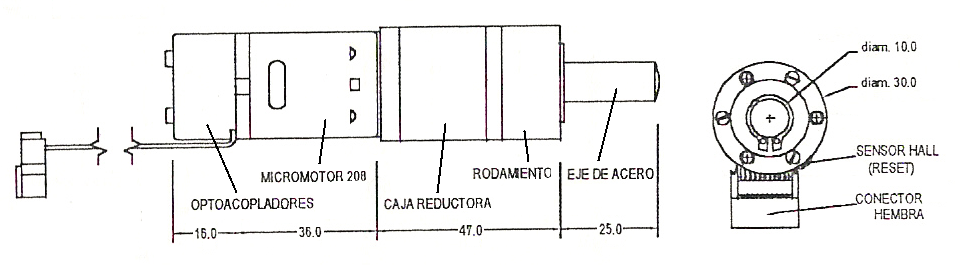
\includegraphics[scale=1]{figuras/MR2-FA.png}
	\caption{Vista lateral y frontal del motor Ignis MR-2FA.}
	\label{hF_motorDC}
\end{figure}

Una ventaja que encontramos en este modelo es que ya trae el encoder integrado aunque su resoluci\'on podr\'ia haber sido mayor.
Los encoders los explicamos m\'as en detalle en la secci\'on \ref{h_sensado_encoder}.
La relaci\'on de la caja reductora es de $94$:$1$.

\paragraph{Circuito de control}
\label{h_actuadores_motorDC_circuito}

Para alimentar y poder controlar los motores elegimos el driver \emph{L298} de la marca ST\footnote{http://www.st.com}.
Internamente tiene dos puentes H puenteables y puede soportar hasta $4 A$.
\'Esto lo logramos teniendo las salidas $1$ y $2$ puenteadas con las salidas $4$ y $3$ respectivamente, como
mostramos en el diagrama de la figura \ref{hF_placa_dc_schema3}.

La principal funci\'on del driver era proveer de la corriente y voltaje necesarios para el funcionamiento del motor, pero la configuraci\'on
del puente H nos di\'o la posibilidad de, con una l\'ogica simple, determinar el sentido de la corriente y potencia que recib\'ia el motor.

Este integrado admite el puenteo de las salidas aumentando as\'i la corriente que circular\'a por el motor.
Para hacer esto, conectamos las salidas \emph{Out1} y \emph{Out4} por un lado y por el otro las salidas \emph{Out2} y \emph{Out3}.
De igual forma los pines de habilitaci\'on \emph{EnA} y \emph{EnB}, luego la entrada \emph{In1} con la \emph{In4} por un lado y
por el otro la \emph{In2} con la \emph{In3}.
De esta forma, lo controlamos con s\'olo $3$ cables, uno de habilitaci\'on y otros $2$ de \emph{Input} que determinan
la polarizaci\'on de los transistores internos y por ende, el sentido de giro del motor.
En el cuadro \ref{hT_l298} mostramos la tabla de verdad para los pines de control, donde H es estado alto, L estado bajo y X cualquier estado.
En la figura \ref{hF_l298} mostramos el diagrama interno del integrado.

\begin{figure}[h]
	\centering
	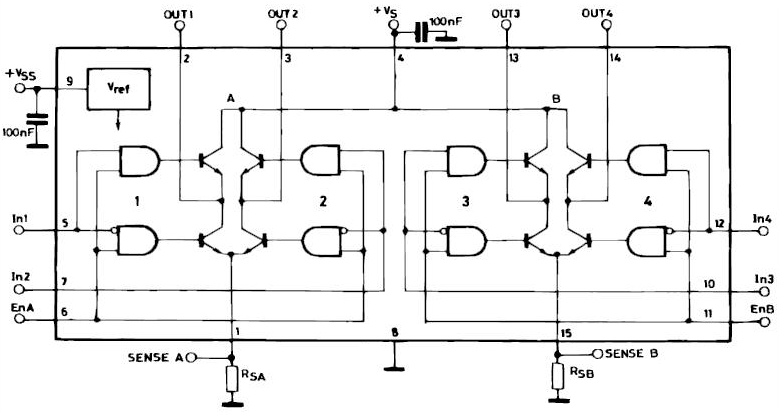
\includegraphics[scale=0.40]{figuras/L298.png}
	\caption{Diagrama interno del driver L298.}
	\label{hF_l298}
\end{figure}

\begin{table}
	\begin{center}
		\begin{tabular}{|c|c|c|c|}
			\hline
			Enable & Input $1$ & Input $2$ & Funci\'on \\
			\hline
			H & H & L & Sentido horario \\
			H & L & H & Sentido anti-horario \\
			H & L & L & Motor frenado \\
			H & H & H & Motor frenado \\
			L & X & X & Motor libre \\
			\hline
		\end{tabular}
	\end{center}
	\caption{Tabla de verdad para el control del driver \emph{L298}.}
	\label{hT_l298}
\end{table}

Para determinar la potencia que recibir\'a el motor usamos el m\'odulo de \emph{PWM} del microcontrolador, que explicamos m\'as en detalle en la
secci\'on \ref{h_controlador_micro_modulos}.
Variando el ancho del pulso sobre el pin de habilitaci\'on del driver determinamos la cantidad de tiempo que el motor recibe tensi\'on, lo cual
se traduce en la potencia que \'este tiene para realizar el movimiento.
Cuanto mayor es el tiempo en estado alto del pulso, mayor la potencia.

Para contrarrestar la corriente negativa en las salidas del driver usamos los diodos \emph{FR304} que cumplen con las especificaciones del driver
con $150$ns de tiempo de recuperaci\'on y una corriente de $3 A$.

El consumo del motor lo medimos mediante los pines de sensado en el driver, conectado a masa por una resistencia y al m\'odulo de \emph{ADC} del
microcontrolador, que explicamos en la secci\'on \ref{h_controlador_micro_modulos}.
Conociendo el valor de la resistencia y el valor le\'ido por el m\'odulo de \emph{ADC}, pudimos determinar cu\'anta corriente que circulaba por la
resistencia y por ende la corriente consumida por el motor.

Para controlar la velocidad del motor usamos uno de los dos encoders que trae.
Conectados como entrada para el m\'odulo de \emph{Timer} del microcontrolador, en configuraci\'on de contador, que explicamos m\'as en detalle en la
secci\'on \ref{h_controlador_micro_modulos}.
Usando otro \emph{Timer} para tener una base de tiempo fija y con el valor del contador pudimos determinar y controlar la velocidad de las ruedas.
Dependiendo el tama\~no de las mismas ser\'a la velocidad de final del robot.

En la secci\'on \ref{h_placas_motorDC} explicamos el desarrollo de la placa controladora de estos motores.

\paragraph{Rutinas de control}
\label{h_actuadores_motorDC_rutinas}

Desde el punto de vista del c\'odigo, tuvimos que desarrollar las rutinas necesarias para el manejo de los motores seg\'un las intrucciones del
controlador principal.

Configuramos a uno de los timers internos del microcontrolador para que genere una interrupci\'on cada $6.25ms$, la cual usamos para realizar
chequeos y ejercer control sobre el motor.
Verificamos el consumo del motor para evitar sobrecargar el circuito y los motores ante un posible atasco de las ruedas.
Tambi\'en actualizamos el acumulado de vueltas realizadas por el motor para la odometr\'ia.

Cada $200$ms ($32$ interrupciones) tomamos la cantidad de cuentas del encoder, corregimos la velocidad de giro del motor ajustando el
ancho del pulso generado por el PWM.
Luego borramos el contador y esperamos otros $200ms$.

\subsubsection{Servo motores}
\label{h_actuadores_servo}

Para el movimiento de las partes del m\'odulo de recolecci\'on, una c\'amara con paneo y giro o un sensor de ultrasonido colocado
en la parte superior haciendo las veces de radar, pensamos en el uso de servo motores.
La principal caracter\'istica de estos actuadores es que s\'olo debemos indicar el \'angulo al que queremos que est\'e
el eje del motor y \'este se coloca autom\'aticamente.
El \'angulo de trabajo va desde $0^{\circ}$ a $180^{\circ}$ y algunos llegan hasta los $200^{\circ}$.

Aunque no fue implementado el ning\'un mecanismo que requiriera el uso de estos motores, explicamos en este apartado el trabajo realizado
en torno a este tipo de actuadores.
En la secci\'on \ref{h_placas_servos} explicamos el dise\~no de las placas que los controlan.

El servo de prueba que utilizamos para el desarrollo es el modelo \emph{HX5010} de la marca Hextronik\footnote{http://www.hextronik.com/}
con caracter\'isticas que expresamos en el cuadro \ref{hT_hx5010}

\begin{table}
	\begin{center}
		\begin{tabular}{|c|c|c|}
			\hline
			Caracter\'istica & Unidad & Valor \\
			\hline
			Torque & kg & $6.5$ \\
			Velocidad & segundos/grado & $\frac{0.16}{60}$ \\
			Voltaje & V & $4.8$ a $6$ \\
			Delay m\'aximo & $\mu s$ & $4$ \\
			Dimensiones & $mm$ & 40x20x38 \\
			Peso & $g$ & $39$ \\
			\hline
		\end{tabular}
	\end{center}
	\caption{Caracter\'isticas del servo HX5010.}
	\label{hT_hx5010}
\end{table}

\paragraph{Circuito de control}
\label{h_actuadores_servo_circuito}

La alimentaci\'on y consumo depende del modelo espec\'ifico, variando tambi\'en el torque que posee el servo.

No es necesario el uso de un driver para manejarlos, simplemente con la alimentaci\'on y una se\~nal con el \'angulo es suficiente.
La forma de comunicar el \'angulo var\'ia entre los distintos servos y fabricantes.
Hay servos anal\'ogicos y servos digitales.
En los primeros la posici\'on se determina mediante un voltaje que var\'ia seg\'un cierto rango y si es digital, se setea mediante el ancho de
un pulso que tiene un tiempo m\'inimo y m\'aximo para mapear los \'angulos m\'inimo y m\'aximo respectivamente.

Dentro del modo de uso, podemos hacer que queden sueltos o que se queden fijos en cierta posici\'on indicando, de forma cont\'inua, el valor
del \'angulo requerido.
La frecuencia a la que debemos setear la posici\'on depende del modelo.

\paragraph{Rutinas de control}
\label{h_actuadores_servo_rutinas}

Debido a que pensamos usar servos digitales y por lo menos \'ibamos a necesitar $3$ servos, necesitabamos contar con varios m\'odulos de PWM.
Como s\'olo dispon\'iamos de 1, decidimos realizar la misma funci\'on pero por software.

Usamos el timer de $16$bits del microcontrolador configurado con el clock interno como medida del tiempo para crear $5$ salidas con
pulsos que var\'ian su ancho en forma independiente cada una.
Definimos un ancho m\'inimo y m\'aximo, pudiendo configurar pasos intermedios de $1^{\circ}$ (aproximadamente $69.4\mu s$).

\subsection{Sensado}
\label{h_sensado}

En este apartado explicamos detalladamente cada uno de los sensores que utilizamos para realizar tanto las mediciones externas como las internas al robot.
Analizamos las ventajas de cada uno, problemas que encontramos y sus soluciones.

En la secci\'on \ref{h_placas_sensado} explicamos el dise\~no y construcci\'on de las placas que controlan todos los sensores del robot.

\subsubsection{Tel\'emetros infrarrojos}
\label{h_sensado_telemetros}

El principio de funcionamiento de estos sensores es mediante un haz de luz infrarroja que es emitido hacia el objetivo, el cual
es reflejado y captado a trav\'es de un lente por un sensor de posici\'on relativa en el interior del sensor.
En base a esta medici\'on calculamos la distancia entre el sensor y el objeto reflectivo que se encuentra frente a \'el.

\paragraph{Caracter\'isticas}
\label{h_sensado_telemetros_caracteristicas}

Los tel\'emetros infrarrojos que elegimos son de la marca Sharp\footnote{http://sharp-world.com/products/device}, modelo \emph{GP2D120}.
En el cuadro \ref{hT_gp2d120} detallamos los valores caracter\'isticos del modelo.

Este tipo de sensores tiene un retardo de aproximadamente $43.1ms$ durante el cual la lectura que realizamos no es confiable y luego
las nuevas lecturas se hacen en ventanas de aproximadamente el mismo tiempo.
En la figura \ref{hF_gp2d120_pulse} mostramos el diagrama de tiempos.

\begin{table}[h]
	\begin{center}
		\begin{tabular}{|l|c|c|}
			\hline
			Caracter\'istica & Unidad & Valor\\
			\hline
			Rango m\'aximo & $cm$ & 30 \\
			Rango m\'inimo & $cm$ & 4 \\
			Tensi\'on para la m\'axima distancia & $V$ & 1.95 \\
			Tensi\'on para la m\'inima distancia & $V$ & 2.55 \\
			Tensi\'on de alimentaci\'on & $V$ & 5 \\
			Consumo m\'aximo & $mA$ & 50 \\
			\hline
		\end{tabular}
	\end{center}
	\caption{Caracter\'isticas del sensor de distancia por ultrasonido SRF05.}
	\label{hT_gp2d120}
\end{table}

\begin{figure}[h]
	\centering
	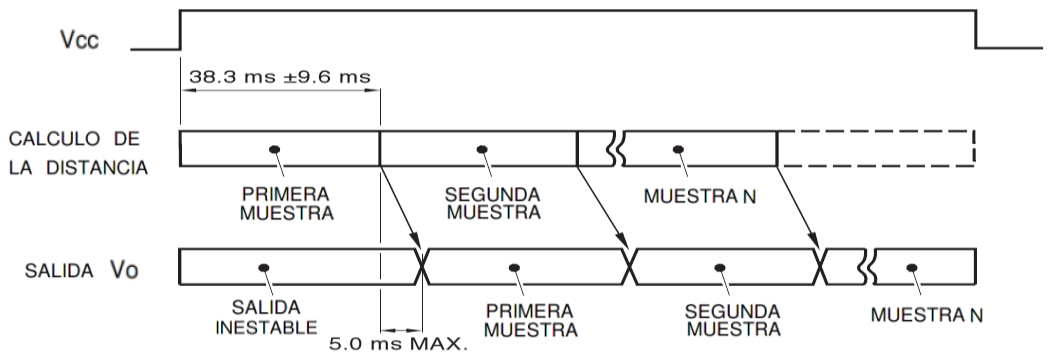
\includegraphics[scale=0.25]{figuras/gp2d120_pulse.png}
	\caption{Diagrama de tiempos del sensor GP2D120.}
	\label{hF_gp2d120_pulse}
\end{figure}

\paragraph{Circuito de control}
\label{h_sensado_telemetros_circuito}

No necesit\'abamos un driver para manejar los tel\'emetros, pero decidimos usar un transistor para poder habilitarlos o no,
de otra manera el sensor estaba tomando mediciones continuamente provocando un consumo de bater\'ia innecesario.
De esta forma s\'olo se enciende cuando se va a utilizar.

El transistor que utilizamos es un conmutador y amplificador de uso general, el \emph{BC327} y por ser de tipo PNP se
exita con un estado bajo, por lo que la l\'ogica de conmutaci\'on est\'a negada.

El tipo de salida de este modelo de tel\'emetros es anal\'ogica y est\'an conectadas al m\'odulo \emph{ADC} del microcontrolador.
En la figura \ref{hF_gp2d120_distancia} mostramos el cuadro de conversi\'on entre voltaje de salida y distancia al objeto, y en la figura
\ref{hF_gp2d120_apertura} mostramos el \'angulo de apertura de la zona de detecci\'on seg\'un la distancia al objetivo.

\begin{figure}[h]
	\begin{minipage}[b]{0.5\linewidth}
		\centering
		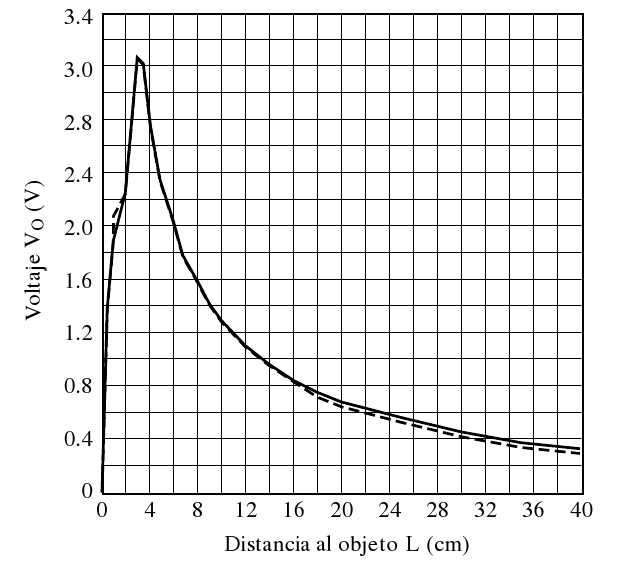
\includegraphics[scale=0.25]{figuras/tel-VxL.png}
		\caption{Voltaje seg\'un la distancia al objeto del tel\'emetro GP2D120.}
		\label{hF_gp2d120_distancia}
	\end{minipage}
	\begin{minipage}[b]{0.5\linewidth}
		\centering
		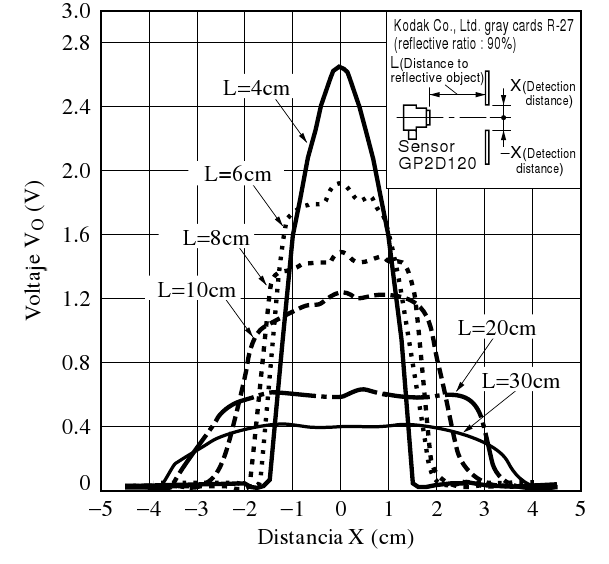
\includegraphics[scale=0.25]{figuras/tel-VxX.png}
		\caption{\'Angulo de apertura seg\'un la distancia del tel\'emetro GP2D120.}
		\label{hF_gp2d120_apertura}
	\end{minipage}
\end{figure}

\paragraph{Rutinas de control}
\label{h_sensado_telemetros_rutinas}

Controlar los tel\'emetros es relativamente sencillo.
Usamos el timer de $16$bits del microcontrolador configurado con el clock interno para determinar el tiempo en el cual
deb\'iamos tomar las muestras con el ADC y simplemente realizamos un promedio entre ellas para obtener la distancia al objetivo.

Para hacer esto desarrollamos una peque\~na m\'aquina de estados que controla y maneja los tiempos para tomar las muestras que
explicamos m\'as en detalle en la secci\'on \ref{h_placas_sensado_codigo}.

\subsubsection{Sensor de distancia por ultrasonido}
\label{h_sensado_ultrasonido}

Estos sensores de distancia se basan en la velocidad del sonido para calcular la distancia al objetivo.
Generan un tren de $8$ pulsos ultras\'onicos y luego se espera como respuesta, el mismo tren de pulsos que deber\'ia haber rebotado contra el objetivo.
En base a la diferencia de tiempo entre la emisi\'on del tren de pulsos y la respuesta, se calcula la distancia a la que se encuentra el objetivo.

\paragraph{Caracter\'isticas}
\label{h_sensado_ultrasonido_caracteristicas}

El sensor de distancia por ultrasonido que elegimos es el modelo \emph{SRF05} de la marca Devantech Ltd\footnote{http://www.robot-electronics.co.uk/}.
Esta versi\'on mejorada del modelo \emph{SRF04}, aumenta el rango de detecci\'on y mejora el modo de control y lectura de los datos, permitiendo
hacerlo mediante un \'unico pin.

La distancia medida mediante el tren de pulsos es codificada linealmente en el ancho de un pulso que var\'ia de $100\mu s$ a $25 ms$.
Si dentro del rango de detecci\'on no se encuentra ning\'un objeto, el pulso tendr\'a un ancho de $30ms$.

En el cuadro \ref{hT_srf05} detallamos las caracter\'sticas del sensor \emph{SRF05} y en la figura \ref{hF_srf05} mostramos el haz ultras\'onico
del sensor.

\begin{table}[h]
	\begin{center}
		\begin{tabular}{|l|c|c|}
			\hline
			Caracter\'istica & Unidad & Valor\\
			\hline
			Tensi\'on de alimentaci\'on & $V$ & 5 \\
			Corriente & $mA$ & 4 \\
			Frecuencia de trabajo & $KHz$ & 40 \\
			Rango m\'aximo & $cm$ & 400 \\
			Rango m\'inimo & $cm$ & 1.7 \\
			Duraci\'on m\'inima del pulso de disparo & $\mu s$ & 10 \\
			Duraci\'on del pulso eco de salida & $\mu s$& 100 - 25000 \\
			Tiempo m\'inimo de espera entre mediciones & $m s$ & 50 \\
			Dimensiones & $mm$ & 43x23x40 \\
			\hline
		\end{tabular}
	\end{center}
	\caption{Caracter\'isticas del sensor SRF05.}
	\label{hT_srf05}
\end{table}

\begin{figure}[h]
	\centering
	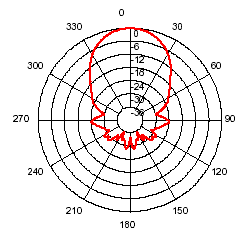
\includegraphics[scale=0.5]{figuras/srf05_beam.png}
	\caption{Haz ultras\'onico del sensor SRF05.}
	\label{hF_srf05}
\end{figure}

\paragraph{Circuito de control}
\label{h_sensado_ultrasonido_circuito}

No necesitamos de un driver para manejar al sensor ya que lo conectamos directo a los $5$ volts de la placa.
El pin de \emph{Mode} lo dejamos en estado bajo para indicar que debe funcionar bajo el nuevo modo y no en compatibilidad con el \emph{SRF04}.

En el pin de \emph{TRIGGER} s\'olo generamos un pulso de al menos $10\mu s$ para desencadenar la lectura de la distancia al objetivo.
El sensor nos asegura que no generar\'a el pulso de respuesta hasta pasados los $700\mu s$ desde pasado el pulso de trigger.
En la figura \ref{hF_srf05_pulse} mostramos el diagrama de tiempos.

\begin{figure}[h]
	\centering
	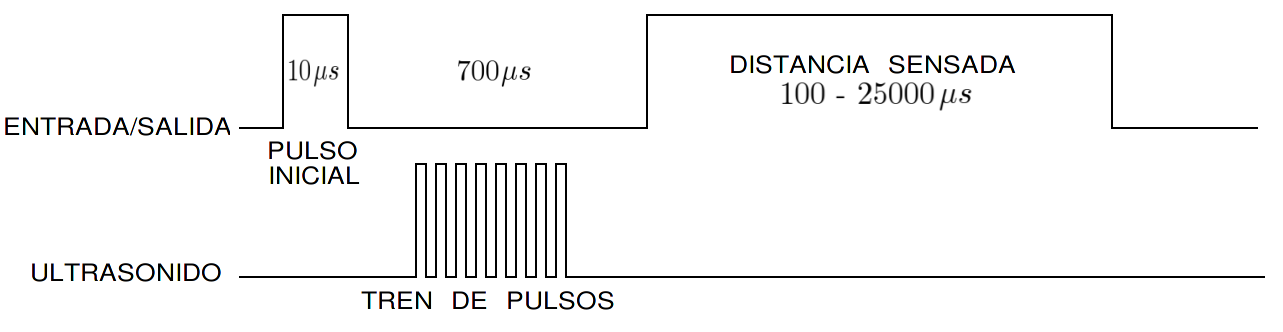
\includegraphics[scale=0.25]{figuras/srf05_pulse.png}
	\caption{Diagrama de tiempos del sensor SRF05.}
	\label{hF_srf05_pulse}
\end{figure}

Para evitar que el rebote de otros sensores o sensados anteriores influya en la lectura, se debe esperar un m\'inimo de $50ms$ antes de
generar otra medici\'on.

\paragraph{Rutinas de control}
\label{h_sensado_ultrasonido_rutinas}

Usamos uno de los pines con interrupci\'on externa en el que conectamos el pin de \emph{TRIGGER} y el timer de $16$bits del microcontrolador
configurado con el clock interno.

Para realizar la medici\'on, generamos un pulso de $15\mu s$ para asegurarnos el disparo del sensor y cambiamos el modo del pin a entrada con
interrupci\'on ante un flanco ascendente.
Cuando salta la interrupci\'on significa que comienza al pulso con la distancia codificada en su ancho, por lo que tomamos una muestra del
timer y configuramos al pin para que genere ahora una interrupci\'on ante un flanco descendente.
Cuando salte la pr\'oxima vez la interrupci\'on, ser\'a porque termin\'o el pulso con la medici\'on, por lo que s\'olo debemos hacer la resta
entre el valor actual del timer y la muestra que tomamos al principio para conocer la distancia a la que se encuentra el objetivo.

Un tiempo obtenido mayor a los $25ms$ indica que no se detect\'o ning\'un objeto dentro del rango del sensor.

\subsubsection{Sensor reflectivo de piso}
\label{h_sensado_piso}

Estos sensores \'opticos reflectivos emiten luz infrarroja y captan el nivel de luz reflejada sobre la superficie a sensar
como mostramos en la figura \ref{hF_cny70_diagrama}.
En la figura \ref{hF_cny70_dim} mostramos las dimensiones del sensor.
La intensidad de luz captada depende de la distancia al objetivo y del color y nivel de reflectividad de la superficie.
Es por esto que usamos estos sensores para identificar una l\'inea en el piso.

\begin{figure}[h]
	\centering
	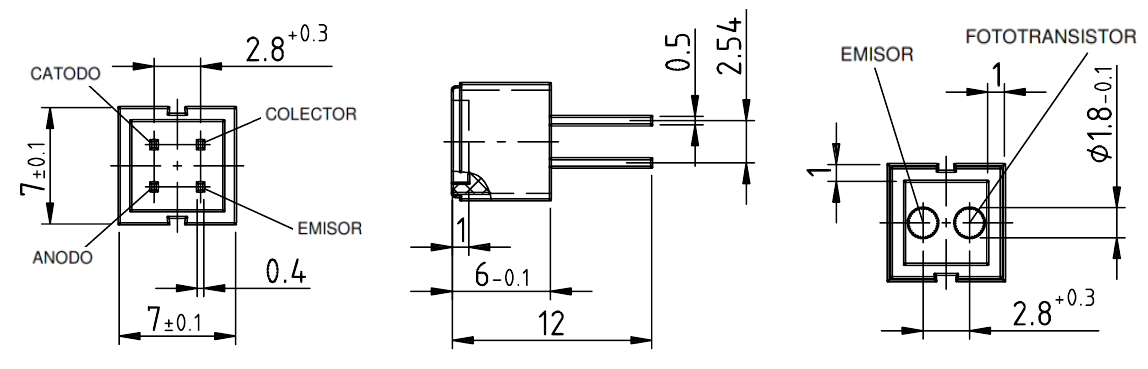
\includegraphics[scale=0.25]{figuras/cny70_dim.png}
	\caption{Medidas en mil\'imetros del sensor CNY70.}
	\label{hF_cny70_dim}
\end{figure}

\paragraph{Caracter\'isticas}
\label{h_sensado_piso_caracteristicas}

Los sensores que elegimos son del modelo \emph{CNY70} de la marca Vishay Semiconductor\footnote{http://www.vishay.com/}.

El rango efectivo de sensado ronda los $3 mm$ de distancia aunque, con un incremento en la corriente que circula por el emisor
se puede llegar a una distancia mayor a la recomendada por el fabricante y que nos permita un uso m\'as acorde al proyecto.
El emisor soporta un pulso de hasta $3 A$ por un tiempo menor o igual a $10\mu s$.

En la figura \ref{hF_cny70_ID} mostramos la corriente que circula por el colector del fototransistor en base a la distancia al objeto medido.

\begin{figure}[h]
	\begin{minipage}[b]{0.45\linewidth}
		\centering
		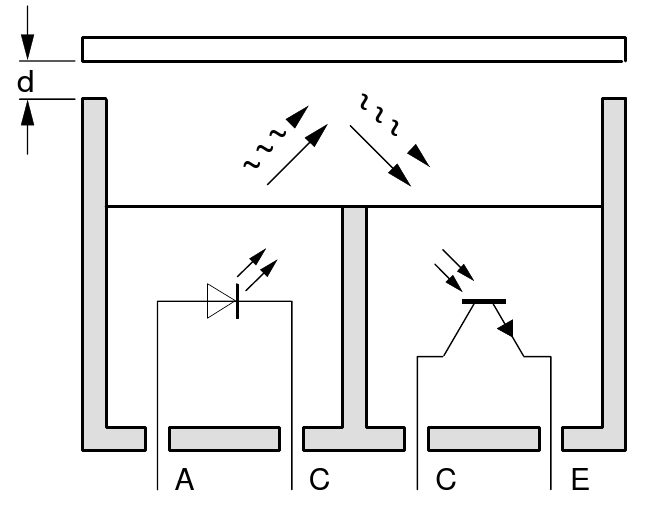
\includegraphics[scale=0.25]{figuras/cny70_diagrama.png}
		\caption{Principio de funcionamiento reflectivo del sensor CNY70.}
		\label{hF_cny70_diagrama}
	\end{minipage}
	\hspace{0.5cm}
	\begin{minipage}[b]{0.45\linewidth}
		\centering
		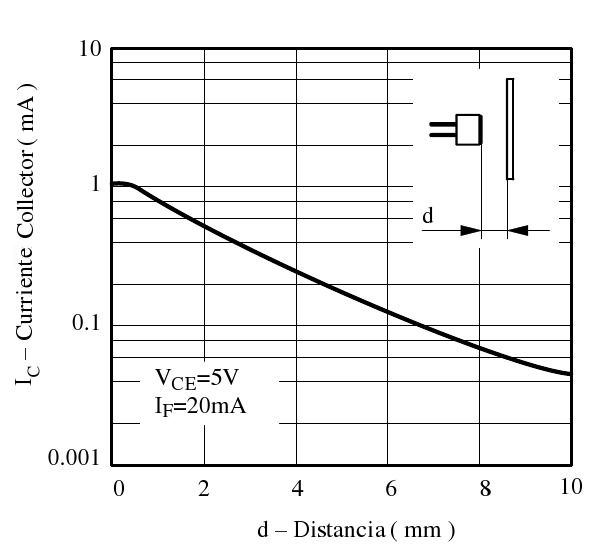
\includegraphics[scale=0.25]{figuras/cny70_IxD.png}
		\caption{Corriente en el colector seg\'un la distancia del sensor CNY70.}
		\label{hF_cny70_ID}
	\end{minipage}
\end{figure}

\paragraph{Circuito de control}
\label{h_sensado_piso_circuito}

De igual forma que en los tel\'emetros utilizamos un transistor como habilitaci\'on de la tensi\'on de alimentaci\'on en el sensor.
Esto nos di\'o la posibilidad de encenderlo y apagarlo a la hora de tomar las muestras de la luz reflejada por piso o la l\'inea.
Nuevamente la l\'ogica de habilitaci\'on es invertida por tratarse de un transistor \emph{BC327}.

Agregamos una resistencia para limitar la corriente que circulaba por el emisor y otra como pull-up en el emisor del fototransistor
que a su vez, conectamos al m\'odulo de \emph{ADC} del microcontrolador para efectuar las mediciones.

\paragraph{Rutinas de control}
\label{h_sensado_piso_rutinas}

El c\'odigo que desarrollamos para obtener las muestras de estos sensores es sencillo, simplemente debemos habilitar el
transistor que alimenta al sensor con un estado l\'ogico bajo, tomar al menos $4$ muestras y promediarlas para tener un
valor adecuado del nivel de luz reflejado por la superficie.
Luego deshabilitamos el sensor y enviamos el valor.

Debido al circuito que armamos con un nivel alto de reflexi\'on leemos un valor bajo en el conversor anal\'ogico digital y
con un nivel bajo de luz, un valor alto.

\subsubsection{Encoders}
\label{h_sensado_encoder}

Los encoders son sensores que convierten una posici\'on lineal o angular en se\~nal el\'ectrica o pulsos.
Pueden determinar una posici\'on de forma absoluta o simplemente informar que hubo un movimiento.
El m\'etodo de sensado y la resoluci\'on del \'angulo de giro que detectan var\'ia seg\'un el modelo.

\paragraph{Caracter\'isticas}
\label{h_sensado_encoder_caracteristicas}

Los motores \emph{MR-2FA} tienen encoders de cuadratura conectados al eje, previo a la caja reductora.
Estos encoders son de tipo fotoel\'ectricos, estan dispuestos a $135^{\circ}$ uno del otro y marcan $4$ estados por
cada vuelta del motor.
El motivo de \'esto es para poder conocer el sentido de giro midiendo la secuencia de estados de cada encoder.
Adicionalmente el motor cuenta con un sensor de efecto Hall el cual nos permite detectar una revoluci\'on completa
en el eje de salida de la caja reductora.

Como conocemos el sentido de giro del motor, pues lo determinamos con el puente H, necesitamos s\'olo
uno de los dos encoders para conocer y controlar la velocidad a la que gira el rotor del motor.

A la tensi\'on m\'axima los motores superan las 320 cuentas por segundo, el m\'inimo y m\'aximo recomendables
son, para que podamos mantener un giro constante, $60$ y $300$ cuentas por segundo respectivamente.
Estos c\'alculos son usando uno de los dos fototransistores del encoder.

\paragraph{Circuito de control}
\label{h_sensado_encoder_circuito}

Conectamos una resistencia pull-up a $5V$ para la salida de sensado de los fototransistores y del
sensor de efecto Hall.
Tambi\'en incluimos un switch doble inversor para elegir cu\'al de los dos encoders usar.
El punto com\'un del switch est\'a conectado al pin de entrada de clock externo de uno de los timers del
microcontrolador.

La alimentaci\'on de los encoders es directa y permanecen encendidos en todo momento.

\paragraph{Rutinas de control}
\label{h_sensado_encoder_rutinas}

Como explicamos en la secci\'on \ref{h_actuadores_motorDC_rutinas}, en cada interrupci\'on del timer actualizamos
el hist\'orico de cuentas del motor adicionando o restando el \'ultimo valor del contador.

Tambi\'en comparamos contra las cuentas esperadas por intervalo de tiempo que fueron determinadas desde el controlador
principal para poder determinar si debemos incrementar o disminuir la potencia del motor y por ende la velocidad de las ruedas.

\subsubsection{Sensado de la bateria}
\label{h_sensado_bateria}

El sensado del nivel de tensi\'on en la bater\'ia lo hacemos mediante un divisor de tensi\'on entre los polos de la bater\'ia.
La salida del divisor es sensada de igual forma que los otros sensores, mediante el m\'odulo de \emph{ADC} del microcontrolador.
En la figura \ref{hF_bateria_diagrama} mostramos el diagrama del divisor de tensi\'on.

\begin{figure}[h]
	\centering
	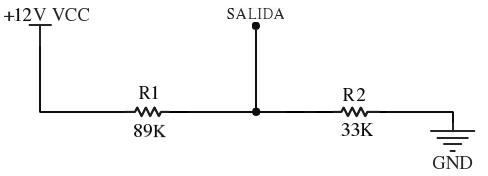
\includegraphics[scale=0.35]{figuras/bateria.png}
	\caption{Divisor de tensi\'on para el sensado de la bater\'ia.}
	\label{hF_bateria_diagrama}
\end{figure}

En el cuadro \ref{hT_bateria_divT} mostramos las posibles tensiones en la bater\'ia y la tensi\'on de salida en el divisor.
Tambi\'en incluimos el valor aproximado para el ADC con tensi\'on de referencia a $5V$ que leer\'ia la salida del divisor.
El rango de voltajes que analizamos es tenendo en cuenta la posibilidad de efectuar mediciones durante la carga de la bater\'ia
y sabiendo que con una tensi\'on menor a $5 V$ la l\'ogica del prototipo que construimos comenzar\'ia a fallar.

\begin{table}[h]
	\begin{center}
		\begin{tabular}{|c|c|c|c|}
			\hline
			Bater\'ia ($V$) & Salida ($V$) & Valor en el ADC \\
			\hline
			16 & 4.327 & 886 \\
			15 & 4.057 & 831 \\
			14 & 3.786 & 776 \\
			13 & 3.516 & 720 \\
			12 & 3.245 & 665 \\
			11 & 2.975 & 609 \\
			10 & 2.704 & 554 \\
			 9 & 2.434 & 499 \\
			 8 & 2.163 & 443 \\
			 7 & 1.893 & 388 \\
			 6 & 1.623 & 332 \\
			 5 & 1.352 & 277 \\
			\hline
		\end{tabular}
	\end{center}
	\caption{Tensi\'on de la bater\'ia y la tensi\'on de salida en el divisor.}
	\label{hT_bateria_divT}
\end{table}

La conexi\'on es simple, los cables de entrada del divisor los conectamos a los polos de la bater\'ia y la salida al ADC.
Luego s\'olo debemos realizar las lecturas en el ADC y promediarlas para poder realizar los c\'alculos de la tensi\'on en la bater\'ia.

\subsubsection{Consumo del motor}
\label{h_sensado_consumo}

El consumo de los motores de corriente cont\'inua lo medimos leyendo el pin de sensado que se encuentra en el puente H que alimenta al motor.
Lo que medimos con el m\'odulo de \emph{ADC} del microcontrolador es la tensi\'on en este pin.
\'Esta depende de la ca\'ida de tensi\'on en la resistencia conectada a masa y de la corriente que circula por el motor.
Conociendo el valor de la resistencia podemos calcular el consumo del motor.
En el cuadro \ref{hT_consumo} comparamos el consumo en el motor, el voltaje sensado y la lectura en el ADC.

\begin{table}[h]
	\begin{center}
		\begin{tabular}{|c|c|c|c|}
			\hline
			Tensi\'on ($V$) & Consumo ($A$) & Valor en el ADC \\
			\hline
			$0$ & $0$ & $0$ \\
			$0.09$ & $0.19$ & $18$ \\
			$0.18$ & $0.38$ & $36$ \\
			$0.27$ & $0.57$ & $55$ \\
			$0.36$ & $0.76$ & $73$ \\
			$0.45$ & $0.95$ & $92$ \\
			$0.54$ & $1.14$ & $110$ \\
			$0.63$ & $1.34$ & $129$ \\
			$0.72$ & $1.53$ & $147$ \\
			$0.81$ & $1.72$ & $165$ \\
			$0.90$ & $1.91$ & $184$ \\
			$0.99$ & $2.10$ & $202$ \\
			$1.08$ & $2.29$ & $221$ \\
			$1.17$ & $2.48$ & $239$ \\
			\hline
		\end{tabular}
	\end{center}
	\caption{Tabla comparativa para el consumo del motor.}
	\label{hT_consumo}
\end{table}

\paragraph{Pulsador u otro dispositivo disparador}
\label{h_sensado_pulsador}

Adem\'as de los sensores que describimos, pensamos que nos podr\'ian hacer falta pulsadores para controlar funciones
simples.
Por ejemplo saber cu\'ando una parte de alg\'un mecanismo llega a cierto punto o detectar finales de carrera
de un servo o tornillo sin fin.
Tambi\'en pueden ser otro tipo de sensores que generen un cambio de estado en el pin de sensado que se conecta al
microcontrolador.

Agregamos la posibilidad de usarlos en las distintas placas como explicamos en detalle en las secciones
\ref{h_placas_sensado} y \ref{h_placas_servos}.

\paragraph{Rutinas de control}
\label{h_sensado_pulsador_rutinas}

La lectura en el estado de los pulsadores puede ser bajo demanda con s\'olo leer el estado del pin en el que est\'an
conectados o puede ser ante una interrupci\'on por cambio de estado.
Estas cuestiones las tuvimos en cuenta a la hora de dise\~nar las placas.

\subsection{Controladores}
\label{h_controlador}

Todas las funciones del robot las deb\'iamos controlar mediante alg\'un tipo de dispositivo.
Decidimos utilizar una netbook y microcontroladores para esta tarea.
Estas cuestiones son las que explicamos en este cap\'itulo.

\subsubsection{Netbook}
\label{h_controlador_netbook}

Elegimos como controlador principal la netbook \emph{EeePC 1005-HA} de la marca Asus\footnote{http://www.asus.com/}.
Como caracter\'isticas principales cuenta con un procesador Intel\footnote{http://www.intel.com/} Atom N280 1.66 GHz,
1GB DDR-2, un disco de 250GB, una pantalla de 10 pulgadas y una bater\'ia de 48Wh que nos da una autonom\'ia de 
aproximadamente 8 horas.
Cuenta con una c\'amara integrada de 0.3MP, placa de red inal\'ambrica y ethernet, placa de sonido y 3 puertos USB.
Pesa aproximadamente 1.27Kg y sus dimensiones son $26.2$ x $17.8$ x $3.7$ cent\'imetros.

Usamos Ubuntu\footnote{http://www.ubuntu.com/} como sistema operativo y programamos tanto la l\'ogica de comportamientos
como la captura y an\'alisis de im\'agenes en C/C++.

\subsubsection{Microcontrolador}
\label{h_controlador_micro}

Para el control de la velocidad de los motores, lectura de los encoders y los sensores de distancia usamos un
microcontrolador.
En nuestro dise\~no contemplamos la existancia de varios m\'odulos con una o pocas funciones simples que se comunicaran
con el controlador principal, que para nuestro prototipo la netbook.
La raz\'on por la cual lo armamos as\'i fue para simplificar cada placa controladora a nivel software y hardware.

Explicamos la comunicaci\'on entre los distintos controladores en la secci\'on \ref{h_comm}.

\paragraph{Caracter\'isticas}
\label{h_controlador_micro_caracteristicas}

El microcontrolador que elegimos para realizar las tareas de control, configuraci\'on y comunicaci\'on a bajo nivel
es el \emph{PIC16F88} de Microchip\footnote{http://www.microchip.com/}.
Cuenta con una arquitectura de memoria del tipo Harvard, con una memoria \emph{FLASH} para 4096 instrucciones de
programa, una memoria \emph{RAM} de 368 bytes y una memoria \emph{EEPROM} de 256 bytes.
Tiene un set de instrucciones b\'asicas reducido y todas con el mismo tiempo de ejecuci\'on.
En este apartado nombramos algunos de los principales perif\'ericos incluidos en el microcontrolador y la utilidad
dentro del proyecto que encontramos para ellos.
Utilizamos con un cristal externo de 20MHz como clock.

\begin{figure}[h]
	\centering
	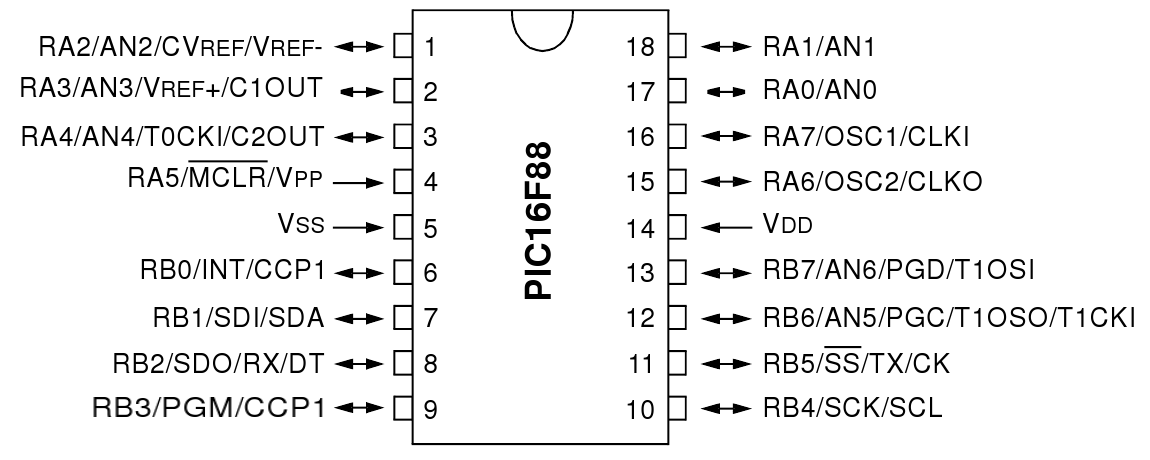
\includegraphics[scale=0.20]{figuras/pic16f88.png}
	\caption{Diagrama del microcontrolador PIC16F88.}
	\label{hF_pic16f88_diagrama}
\end{figure}

El microcontrolador tiene 2 puertos de 8 entradas y salidas cada uno de tipo TTL y CMOS.
Como mostramos en la figura \ref{hF_pic16f88_diagrama} cada pin se encuentra multiplexado con uno o m\'as perif\'ericos internos.

\paragraph{M\'odulos internos}
\label{h_controlador_micro_modulos}

Internamente el microcontrolador tiene una serie de perif\'ericos que proveen funciones extras y que utilizamos para lograr
cumplir con las necesidades de nuestro proyecto.
En la figura \ref{hF_pic16f88_modulos} mostramos los distintos m\'odulos internos del microcontrolador.

\begin{figure}[b]
	\centering
	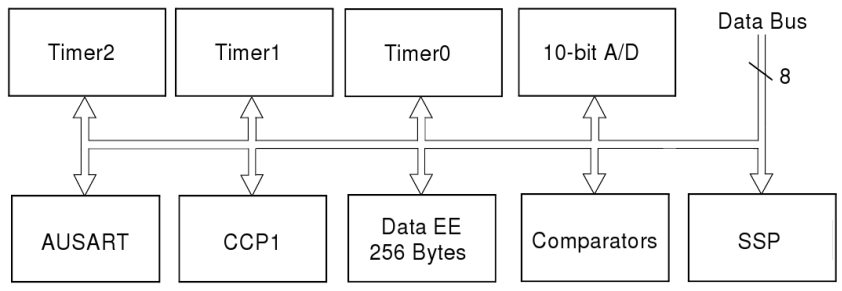
\includegraphics[scale=0.35]{figuras/pic16f88_modulos.png}
	\caption{M\'odulos internos del microcontrolador PIC16F88.}
	\label{hF_pic16f88_modulos}
\end{figure}

Cuenta con $3$ timers, $2$ de $8$bits (\emph{TIMER0} y \emph{TIMER2}) y $1$ de $16$bits (\emph{TIMER1}).
Podemos configurarlos para que tomen al clock del microcontrolador o que tomen una fuente externa de clock.
Tambi\'en podemos aplicarles demultiplicadores que generan un clock de menor frecuencia al que se usa como entrada.
Pueden ser etapas previas o posteriores al timer y nos dan gran flexibilidad de uso.

El \emph{TIMER0} lo utilizamos para hacer control del tiempo en nuestros c\'odigos.
Conectados con el clock principal y configurados para que generen una interrupci\'on al hacer overflow,
obtenemos una buena medida del paso del tiempo.

El \emph{TIMER1} configurado como fuente externa a la salida del encoder, lo usamos como contador de pasos para medir la
velocidad del motor.
Tambi\'en lo usamos como medici\'on del tiempo para hacer las lecturas de los sensores.
Elegimos a este timer ya que al ser de $16$bits posee un mayor rango de valores y por lo tanto, pod\'iamos medir un mayor lapso
de tiempo o cuentas del encoder en cada caso.

El \emph{TIMER2} lo usamos en conjunto con el m\'odulo de \emph{PWM} para determinar el ancho del pulso que habilita al puente H
que provee de energ\'ia a los motores.

El m\'odulo conversor anal\'ogico digital nos di\'o la posibilidad de medir tensiones anal\'ogicas como por ejemplo
las salidas de los sensores, tensi\'on en la bater\'ia o el consumo de los motores.
Tiene $7$ canales o pines distintos y podemos configurarlo para que genere un valor de $8$ o $10$bits.
Tambi\'en podemos determinar si se debe usar el valor de \emph{Vcc} y \emph{GND} como referencia o podemos proveer
de forma externa de los voltajes de referencia para generar un rango de voltajes diferente y aumentar o disminuir
as\'i la resoluci\'on del conversor.

El m\'odulo de \emph{PWM} nos provee la posibilidad de generar pulsos cont\'inuos de un ancho determinado.
En nuestro proyecto lo utilizamos como habilitaci\'on del puente H que alimenta a los motores variando as\'i la
potencia y por lo tanto, la velocidad final de las ruedas.
Se utiliza en conjunto con el \emph{TIMER2} seteando el prescaler y postscaler para determinar el ancho del
estado alto y del estado bajo de los pulsos.

Gracias al m\'odulo de \emph{AUSART} podemos realizar la comunicaci\'on entre los distintos microcontroladores por hardware.
Este perif\'erico nos provee una conmunicaci\'on sincr\'onica o asincr\'onica dependiendo de la configuraci\'on.
Creamos la red de \emph{Daisy-Chain} sobre el protocolo de RS-232.

El microcontrolador dispone de otros perif\'ericos como un comparador \emph{CCP} y comunicaci\'on sincr\'onica \emph{SPI}.
Utilizamos los pines de uso general para realizar otras funciones como habilitaci\'on, conmutaci\'on o las se\~nales de
\emph{PWM} por software para determinar la posici\'on de los servo motores, por ejemplo.

\paragraph{Programaci\'on del firmware}
\label{h_controlador_micro_programacion}

Para crear el firmware de cada microcontrolador usamos al IDE de programaci\'on 
\emph{Microchip MPLAB}\footnote{http://www.microchip.com/}.
Usamos el lenguaje C y lo compilamos con \emph{CCS PCM V4.023}\footnote{http://www.ccsinfo.com/}.
Usamos el programador \emph{ICD2} de la empresa \emph{Microchip} para descargar c\'odigo compilado al microcontrolador.
El cual. a su vez, nos di\'o la posibilidad de depurar el c\'odigo en m\'as de una oportunidad.

En el cuadro \ref{hT_header_icd2} detallamos el header de programaci\'on en circuito, con el cual establecemos la
interface con el programador \emph{ICD2} para cargar el firmware en el microcontrolador o para depurarlo.

\begin{table}
	\begin{center}
		\begin{tabular}{|c|c|}
			\hline
			Pines & Se\~nal \\
			\hline
			1 y 2 & MCLR \\
			\hline
			3 y 4 & $5V$ VCC \\
			\hline
			5 y 6 & GND \\
			\hline
			7 y 8 & PGD (Data) \\
			\hline
			9 y 10 & PGC (Clock) \\
			\hline
		\end{tabular}
		\caption{Pines de programaci\'on en circuito con \emph{ICD2}.}
		\label{hT_header_icd2}
	\end{center}
\end{table}


\subsection{Comunicaci\'on}
\label{h_comm}

La comunicaci\'on interna entre los controladores de cada perif\'erico y el controlador principal, donde concentramos
la l\'ogica de los comportamientos, era vital.
Para poder tomar las decisiones adecuadas la telemetr\'ia deb\'ia tener toda la informaci\'on requerida, la frecuencia
suficiente para que las reacciones sean lo m\'as din\'amicas y r\'apidas posibles y poseer la menor cantidad de errores
para evitar retransmisiones.

En esta secci\'on analizamos todo lo referente al medio de transmisi\'on, protocolo y comandos que forman parte de la
comunicaci\'on interna entre m\'odulos.

\subsubsection{Conectividad entre m\'odulos}
\label{h_comm_conectividad}

Para establecer el canal de comunicaciones decidimos emplear una configuraci\'on basada en el m\'etodo
\emph{Daisy-Chain}\footnote{Patente US20090316836A1} entre los controladores.
Creando un anillo donde cada nodo de la cadena se comunica con su vecino retransmitiendo cada paquete
hasta su destinatario como mostramos en la figura \ref{hF_comm_daisychain}.

\begin{figure}[h]
	\centering
	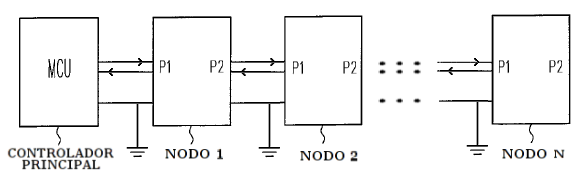
\includegraphics[scale=.40]{figuras/daisychain_diagram.png}
	\caption{Diagrama general del m\'etodo Daisy-Chain}
	\label{hF_comm_daisychain}
\end{figure}

La configuraci\'on que elegimos para realizar la comunicaci\'on fue una velocidad de $115200$ baudios, $8$ bits, con $1$
bit de parada, sin bit de paridad y sin control de flujo.
Logramos una gran velocidad de respuesta a los comandos de esta forma.

En los cuadros \ref{hT_comm_conexionLink} y \ref{hT_comm_conexionRS232} especificamos el conexionado entre las placas
y contra el controlador principal.

\begin{table}[h]
	\begin{center}
		\begin{tabular}{|c|c|c|c|}
			\hline
			Funci\'on & Conector RJ11 & Conector RJ11 & Funci\'on\\
			\hline
			Serial RX & 2 & 2 & Serial TX \\
			\hline
			Serial TX & 3 & 3 & Serial RX \\
			\hline
			No conectado & 4 & 4 & No conectado \\
			\hline
			GND & 5 & 5 &  GND\\
			\hline
		\end{tabular}
		\caption{Conexionado entre placas en modo Link}
		\label{hT_comm_conexionLink}
	\end{center}
\end{table}

\begin{table}[h]
	\begin{center}
		\begin{tabular}{|c|c|c|c|}
			\hline
			Funci\'on & Conector RJ11 & Conector DB9 & Funci\'on\\
			\hline
			Serial RX & 2 & 3 & Serial TX \\
			\hline
			Serial TX & 3 & 2 & Serial RX \\
			\hline
			No conectado & 4 & 4 & Shield \\
			\hline
			GND & 5 & 5 &  GND\\
			\hline
		\end{tabular}
		\caption{Conexionado entre placa y la PC}
		\label{hT_comm_conexionRS232}
	\end{center}
\end{table}

Como terminaci\'on de la cadena, debemos colocar una ficha nula que interconecte \emph{TX} con \emph{RX} o
cambiar el switch de configuraci\'on de \emph{LINK} a \emph{LAST}.

\subsubsection{Protocolo de comunicaci\'on}
\label{h_comm_protocolo}

El protocolo de comuncaci\'on est\'a formado por paquetes que tienen un formato espec\'ifico y representan un pedido de
informaci\'on o comando que debe ser ejecutado en el destino.

El paquete consta de un header com\'un con datos que identifican al emisor y receptor del paquete, el comando a enviar y
posibles datos extras que sean requeridos.
Todos los paquetes tienen una respuesta obligatoria de confirmaci\'on de recepci\'on.
Cuando el paquete requiere una respuesta con datos, la confirmaci\'on va acompa\~nada de la informaci\'on requerida.
En el cuadro \ref{hF_comm_paquete_tabla} mostramos la estructura interna de un paquete t\'ipico.

\begin{table}[h]
	\begin{center}
		\begin{tabular}{|c|c|c|c|c|c|}
			\hline
			LARGO & DESTINO & ORIGEN & COMANDO & DATO & CRC \\
			\hline
		\end{tabular}
	\caption{Formato y header del paquete de datos}
	\label{hF_comm_paquete_tabla}
	\end{center}
\end{table}

Tanto los paquetes de env\'io de datos como los de respuesta tienen el mismo formato y comparten el valor en el campo de comando.

El campo \emph{LARGO} indica el tama\~no en bytes del paquete que viene a continuaci\'on, consta de 1 byte.
Es necesario porque el campo \emph{DATO} es de longitud variable.
Si la longitud del campo \emph{DATO} es cero, entonces \emph{LARGO} es 0x04.

El campo \emph{DESTINO} identifica al destinatario del paquete y consta de 1 byte.
Los 4 bits m\'as significativos indican el grupo y los 4 bits menos significativos, el n\'umero de $ID$ de la placa de destino.
Si el $ID$ de placa es F, el paquete es broadcast a todos los $ID$s del grupo indicado y si el valor es 0xFF, el paquete
es broadcast a todas las placas de todos los grupos.
En el cuadro \ref{hT_comm_protocolo_grupos} establecemos el $ID$ de cada grupo.

De igual forma, \emph{ORIGEN} determina el emisor del paquete para la respuesta y es de 1 byte.
Los 4 bits m\'as significativos indican el grupo y los 4 bits menos significativos, el n\'umero de $ID$ de la placa de origen.
Los valores permitidos son del $0$ al E, ya que F indica broadcast y no es v\'alida una respuesta broadcast.

El campo \emph{COMANDO} informa al destinatario la tarea a realizar o determina un pedido de informaci\'on que puede o no
tener par\'ametros.
Ocupa 1 byte.

El campo \emph{DATO} contiene los par\'ametros o datos extras que puedan ser necesarios para el comando enviado.
En el caso que el comando no los requiera, el campo debe ser nulo y el campo \emph{LARGO} ser\'a 0x04.

El control de errores lo realizamos mediante un checksum calculado, haciendo un \emph{XOR} con cada byte del contenido del paquete
y coloc\'andolo en el campo \emph{CRC}.
Cuando un paquete se encuentre con errores o est\'e mal formado, el destinarario deber\'ia pedir la retrasmisi\'on.
De igual forma, cre\'imos necesaria la creaci\'on de un control adicional por medio de una lista de paquetes no confirmados mantenida
por el controlador principal para evitar la p\'erdida de comandos.

Para m\'as referencias recomendamos ver el apartado \ref{hA_protocolo}.

\begin{table}[h]
	\begin{center}
		\begin{tabular}{|l|c|}
			\hline
			Grupo & ID \\
			\hline
			MAIN CONTROLLER & 0x00 \\
			\hline
			DC MOTOR & 0x10 \\
			\hline
			SERVO MOTOR & 0x20 \\
			\hline
			DISTANCE SENSOR & 0x30 \\
			\hline
			BATTERY CONTROLLER & 0x40 \\
			\hline
			TRASH BIN & 0x50 \\
			\hline
			-BROADCAST- & 0xF0 \\
			\hline
		\end{tabular}
		\caption{ID para cada grupo seg\'un su funci\'on.}
		\label{hT_comm_protocolo_grupos}
	\end{center}
\end{table}

\paragraph{Comandos comunes}
\label{h_comm_protocolo_comandosComunes}

Creamos comandos que son comunes a cualquier placa sea cual sea su grupo.
La intenci\'on fue poder tener un espacio de comunicaci\'on com\'un para poder intercambiar comandos
de inicializaci\'on, identificaci\'on de controladores, versionado o alg\'una otra necesidad gen\'erica que
se desarrolle en un futuro y deba ser incluida en el protocolo.
El controlador principal deber\'ia ser quien env\'ia este tipo de comandos, pero no creamos restricciones al respecto.

En el cuadro \ref{hT_comm_comandos_comunes} listamos y explicamos brevemente los comandos comunes del protocolo.

\begin{table}[h]
	\begin{center}
		\begin{tabular}{|l|l|p{8.5cm}|}
		\hline
		Valor & Comando & Detalle \\
		\hline
		0x01 & INIT & Sincroniza el inicio de todas las placas en la cadena.
		Responde con los datos necesarios para identificar a la placa en la cadena. \\
		\hline
		0x02 & RESET & Pide el reset de la tarjeta.
		Responde de igual forma que a \emph{INIT}. \\
		\hline
		0x03 & PING & Envia un ping a la placa.\\
		\hline
		0x04 & ERROR & Informa que ha habido un error.
		M\'as informaci\'on sobre el error viaja en el campo de \emph{DATO} y
		depende del grupo de origen. \\
		\hline
		\end{tabular}
		\caption{Comandos comunes a todos los controladores. }
		\label{hT_comm_comandos_comunes}
	\end{center}
\end{table}

\paragraph{Comandos espec\'ificos}
\label{h_comm_protocolo_comandosEspecificos}

Cada grupo de placas tiene comandos propios y espec\'ificos dependiendo de la funci\'on que deban desempe\~nar en el sistema.
Existen grupos con comandos predefinidos cada uno se trata en las secciones como se detalla en el cuadro \ref{hT_comm_protocolo_grupos}.
Los comandos espec\'ificos para cada grupo deben estar dentro del rango de valores entre 0x40 y 0x7E.

El \emph{MAIN CONTROLLER} no posee por ahora ning\'un comando espec\'ifico pero le reservamos el espacio en el protocolo.
En el cuadro \ref{hT_comm_comandos_motordc} enumeramos los comandos para el controlador \emph{DC MOTOR}.
El controlador \emph{SERVO MOTOR} responde a los comandos del cuadro \ref{hT_comm_comandos_servo}.
En el cuadro \ref{hT_comm_comandos_distance} listamos los comandos del controlador \emph{DISTANCE SENSOR}.
De igual forma, aunque no est\'en implementados, reservamos y especificamos los comandos para \emph{BATTERY CONTROLLER} y
\emph{TRASH BIN} en los cuadros \ref{hT_comm_comandos_bateria} y \ref{hT_comm_comandos_basura} respectivamente.

\begin{table}
	\begin{center}
		\begin{tabular}{|l|p{2.5cm}|p{7.5cm}|}
		\hline
		Valor & Comando & Detalle \\
		\hline
		0x40 & SET DIRECTION & Seteo del sentido de giro del motor.
		Env\'ia el sentido de giro como par\'ametro. \\
		\hline
		0x41 & SET DC SPEED & Seteo de la velocidad del motor.
		Env\'ia el sentido de giro y velocidad en cuentas por segundos como par\'ametro. \\
		\hline
		0x42 & SET ENCODER & Seteo de las cuentas hist\'oricas del encoder.
		Env\'ia como par\'ametro el valor para setear en el hist\'orico del encoder. \\
		\hline
		0x43 & GET ENCODER & Obtener las cuentas hist\'oricas del encoder.
		Responde con el valor hist\'orico del encoder. \\
		\hline
		0x44 & RESET ENCODER & Resetear las cuentas hist\'oricas a cero. \\
		\hline
		0x45 & SET ENCODER TO STOP & Seteo de cu\'antas cuentas para detenerse.
		Env\'ia como par\'ametro la cantidad de cuentas del encoder restantes para
		que el motor se detenga. \\
		\hline
		0x46 & GET ENCODER TO STOP & Obtener las cuentas restantes hasta detenerse.
		Responde con la cantidad de cuentas del encoder restantes para que el motor se detenga. \\
		\hline
		0x47 & DONT STOP & Deshabilita el conteo de cuentas para frenar. \\
		\hline
		0x48 & MOTOR CONSUMPTION & Consulta sobre el consumo actual del motor.
		Responde con el consumo promedio del \'ultimo segundo. \\
		\hline
		0x49 & MOTOR STRESS ALARM & Alarma sobre un consumo extremo en el motor.
		Responde con el consumo ante el cu\'al se dispar\'o la alarma. \\
		\hline
		0x4A & MOTOR SHUT DOWN ALARM & Alarma informando que el motor se apag\'o.
		Env\'ia el consumo ante el que se dispar\'o la alarma. \\
		\hline
		0x4B & GET DC SPEED & Obtiene la velocidad en cuentas del encoder por segundo.
		Env\'ia el sentido y velocidad de giro del motor. \\
		\hline
		\end{tabular}
		\caption{Comandos espec\'ificos al \emph{DC MOTOR}.}
		\label{hT_comm_comandos_motordc}
	\end{center}
\end{table}

\begin{table}
	\begin{center}
		\begin{tabular}{|l|p{2.5cm}|p{7.5cm}|}
		\hline
		Valor & Comando & Detalle \\
		\hline
		0x40 & SET POSITION & Determina la posici\'on del servo motor indicado.
		Env\'ia el $ID$ del servo y la posici\'on del eje como par\'ametro. \\
		\hline
		0x41 & SET ALL POSITIONS & Setea las posiciones de cada uno de los servo motores.
		Env\'ia las posiciones para cada uno de los $5$ servos como par\'ametro.\\
		\hline
		0x42 & GET POSITION & Obtiene la \'ultima posici\'on del servo motor indicado.
		Env\'ia como par\'ametro el $ID$ del servo del que se quiere la posici\'on y
		recibe el $ID$ del servo y la posici\'on del eje. \\
		\hline
		0x43 & GET ALL POSITIONS & Obtiene todas las \'ultimas posiciones de los servo motor.
		Responde con la posici\'on para cada uno de los $5$ servos.\\
		\hline
		0x44 & SET SERVO SPEED & Setea la velocidad para el servo motor indicado.
		Env\'ia como par\'ametro el $ID$ del servo y la velocidad a setear. \\
		\hline
		0x45 & SET ALL SPEEDS & Setea la velocidad para cada servo motor.
		Env\'ia como par\'ametro la velocidad a setear para cada uno de los servos. \\
		\hline
		0x46 & GET SERVO SPEED & Obtiene la velocidad para el servo motor indicado.
		Env\'ia como par\'ametro el $ID$ del servo y responde con $ID$ y velocidad del servo. \\
		\hline
		0x47 & GET ALL SPEEDS & Obtiene las velocidades de cada uno de los servo motores.
		Responde con la velocidad de cada uno de los servo motores. \\
		\hline
		0x48 & FREE SERVO & Deja de aplicar fuerza sobre el servo indicado.
		Env\'ia como par\'ametro el $ID$ del servo a liberar.\\
		\hline
		0x49 & FREE ALL SERVOS & Deja de aplicar fuerza sobre cada uno de los servo motores. \\
		\hline
		0x4A & GET STATUS & Obtiene el estado de cada uno de los switches.
		Responde con la 1 byte con el estado de cada switch. \\
		\hline
		0x4B & ALARM ON STATE & Establece si se desea recibir alarmas por cambio de estado.
		Env\'ia como par\'ametro el $ID$ y tipo de cambio en el switch.\\
		\hline
		0x4C & SWITCH ALARM & Alarma ante un cambio de estado programado.
		Env\'ia como par\'ametro el $ID$ y estado del switch que provoc\'o el comando. \\
		\hline
		\end{tabular}
		\caption{Comandos espec\'ificos al \emph{SERVO MOTOR}. }
		\label{hT_comm_comandos_servo}
	\end{center}
\end{table}

\begin{table}[h]
	\begin{center}
		\begin{tabular}{|l|p{2.5cm}|p{7.5cm}|}
		\hline
		Valor & Comando & Detalle \\
		\hline
		0x40 & ON DISTANCE SENSOR & Enciende el sensor de distancia enviado como par\'ametro. \\
		\hline
		0x41 & OFF DISTANCE SENSOR & Apaga el sensor de distancia enviado como par\'ametro. \\
		\hline
		0x42 & SET DISTANCE SENSORS MASK & Habilita o no los sensores para lecturas.
		Env\'ia 1 bit por cada $ID$ del sensor a habilitar o deshabilitar.\\
		\hline
		0x43 & GET DISTANCE SENSORS MASK & Obtiene la m\'ascara de lectura.
		Responde con 1 bit por cada $ID$ del sensor.\\
		\hline
		0x44 & GET VALUE & Obtiene el valor promedio de la entrada de los sensores indicados.
		Env\'ia 1 bit por cada $ID$ del sensor y responde con los valores de lectura promedio de cada sensor. \\
		\hline
		0x45 & GET ONE VALUE &Obtiene el valor de la entrada del sensor indicado.
		Env\'ia 1 bit por cada $ID$ del sensor y responde con los valores de lectura de cada sensor. \\
		\hline
		0x46 & ALARM ON STATE & Setea el tipo de cambio de estado del switch para la alarma.
		Env\'ia como par\'ametro el tipo de cambio de estado.\\
		\hline
		0x47 & SWITCH ALARM & Alarma informando que fue satisfecha la condici\'on.
		Env\'ia como par\'ametro el tipo de cambio y estado actual del switch.\\
		\hline
		\end{tabular}
		\caption{Comandos espec\'ificos al \emph{DISTANCE SENSOR}. }
		\label{hT_comm_comandos_distance}
	\end{center}
\end{table}

\begin{table}[h]
	\begin{center}
		\begin{tabular}{|l|p{2.5cm}|p{7.5cm}|}
		\hline
		Valor & Comando & Detalle \\
		\hline
		0x40 & ENABLE & Habilita la alimentaci\'on del robot mediante la bater\'ia. \\
		\hline
		0x41 & DISABLE & Deshabilita la alimentaci\'on del robot mediante la bater\'ia. \\
		\hline
		0x42 & GET BATTERY VALUE & Obtiene el valor de la entrada de la bater\'ia.
		Responde con la lectura de la tensi\'on en la bater\'ia. \\
		\hline
		0x43 & BATTERY FULL ALARM & Mensaje informando que se completado la carga. \\
		\hline
		0x44 & SET BATTERY EMPTY VALUE & Valor de la bater\'ia cr\'itico.
		Env\'ia la lectura de los volts de la bater\'ia. \\
		\hline
		0x45 & BATTERY EMPTY ALARM & El voltaje lleg\'o a un valor cr\'itico.
		Env\'ia la lectura de los volts de la bater\'ia. \\
		\hline
		0x46 & SET FULL BATTERY VALUE & Establece el valor para la carga completa.
		Env\'ia la lectura de la tensi\'on en la bater\'ia. \\
		\hline
		\end{tabular}
		\caption{Comandos espec\'ificos al \emph{BATTERY CONTROLLER}. }
		\label{hT_comm_comandos_bateria}
	\end{center}
\end{table}

\begin{table}[h]
	\begin{center}
		\begin{tabular}{|l|p{2.5cm}|p{7.5cm}|}
		\hline
		Valor & Comando & Detalle \\
		\hline
		0x40 & GET TRASH BIN VALUE & Consulta que tan lleno est\'a el cesto de basura.
		Responde con el valor que representa el estado del cesto interno. \\
		\hline
		0x41 & BIN FULL ALARM & El cesto de basura se ha completado y debe ser descargado. \\
		\hline
		0x42 & SET FULL BIN VALUE & Setea el valor para determinar que el cesto est\'a lleno.
		Valor que especifica que lectura se debe tomar como cesto lleno.\\
		\hline
		\end{tabular}
		\caption{Comandos espec\'ificos al \emph{TRASH BIN}. }
		\label{hT_comm_comandos_basura}
	\end{center}
\end{table}

% \paragraph{Estad\'isticas}
% \label{h_comm_protocolo_estadisticas}
% 
% analisis de paquetes por segundo, bytes de datos vs bytes de header, retransmisiones, etc

\subsection{Placas controladoras}
\label{h_placas}

Las funciones y requerimientos de nuestro proyecto ten\'ian partes que eran comunes a otros trabajos en rob\'otica o quiz\'as
de electr\'onica general.
Pero ten\'ian peculiaridades y aspectos que no pudimos satisfacer con placas prefabricadas.
Por ejemplo, un protocolo de comunicaci\'on unificado entre todos los m\'odulos era, de entrada, una barrera que acotaba
las posibilidades.
Y mantener distintos modos y protocolos dentro del proyecto generaba una carga de l\'ogica que pod\'iamos evitar.

Analizando las posibilidades y entendiendo que una de las principales razones de nuestro trabajo era generar las bases
de conocimiento y el punto de partida a un proyecto m\'as grande, decidimos producir nuestra propia versi\'on
de placas controladoras.

Aunque iban a tener un uso bien definido dentro de nuestro trabajo, tambi\'en cre\'imos necesario que tuvieran un nivel
de generalidad suficiente como para poder utilizarlas en otros proyectos con m\'inimos cambios, adelantando as\'i mucho
trabajo a futuro.

La modularizaci\'on fue un factor importante y muy presente durante todo el desarrollo.
En este apartado explicamos el dise\~no, desarrollo, programaci\'on y especificaciones de las distintas placas que creamos
durante nuestro proyecto.

\subsubsection{Placa gen\'erica}
\label{h_placas_generica}

Durante el dise\~no nos surgi\'o la necesidad de establecer un m\'odulo com\'un de comunicaci\'on y una base de prueba para
los tests con los distintos sensores y perif\'ericos que utilizar\'iamos en el robot.
Es por \'esto que luego de pruebas aisladas, creamos una placa para estas cuestiones.
Nos ayud\'o y aceler\'o en gran medida el dise\~no de las placas definitivas y nos di\'o la posibilidad de dise\~nar futuras
actualizaciones a nuestro proyecto.

\paragraph{Caracter\'isticas principales}
\label{h_placas_generica_caracteristicas}

La necesidad principal era proveer de una interface com\'un entre todas las placas para la comunicaci\'on y exportar
los puertos y perif\'ericos del microcontrolador que elegimos a circuitos nuevos.
\'Esto nos servi\'o para realizar pruebas de concepto para la conexi\'on con los sensores, valores de componente pasivos
ideales, comportamiento e interacci\'on entre placas, optimizaci\'on del c\'odigo del firmware o crear nuevas expansiones.

\paragraph{M\'odulo de comunicaci\'on}
\label{h_placas_generica_comm}

Como explicamos en la secci\'on \ref{h_comm} para la comunicaci\'on nos basamos en el modelo de \emph{Daisy-Chain} sobre una
capa de transporte de \emph{RS232}.

Los conectores y configuraci\'on son comunes y utilizamos dos tipos de conectores para realizar la interconexi\'on entre las placas.
Como mostramos en la figura \ref{hF_placa_gen_comm} usamos conectores \emph{RJ11} para generar el lazo entre nodos de la cadena y el
conector \emph{DB9} para la conexi\'on con la PC.
En los cuadros \ref{hT_comm_conexionLink} y \ref{hT_comm_conexionRS232} explicamos, respectivamente, el conexionado para cada caso.

\begin{figure}[h]
	\centering
	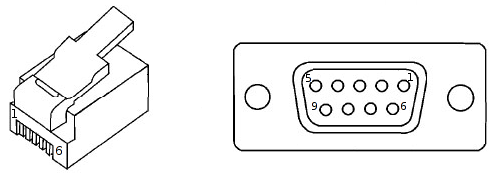
\includegraphics[scale=.25]{figuras/rj11_db9.png}
	\caption{Conectores RJ11 (6P4C) y DB9.}
	\label{hF_placa_gen_comm}
\end{figure}

Para determinar si la placa es un nodo m\'as dentro de la cadena o es la terminaci\'on, colocamos una llave de dos posiciones
que setea la configuraci\'on.
En la posici\'on \emph{LINK} la placa act\'ua como nodo intermedio y en la posici\'on \emph{LAST} como terminaci\'on.

Es de vital importancia colocar en forma la correcta esta llave porque podemos dejar sin conexi\'on al resto de las placas o mismo
perder todos los paquetes transmitidos al no cerrar la cadena en el final de la misma.

\paragraph{Alimentaci\'on de la placa}
\label{h_placas_generica_alimentacion}

La alimentaci\'on principal de la placa es 7 a 20 volts, con la posibilidad de alimentarla directamente con 5 volts
por uno de los pines del conector.
En la figura \ref{hF_placa_gen_borneras} mostramos la bornera y en el cuadro \ref{hT_placa_gen_alimentacion} el pinout.

\begin{figure}[h]
	\centering
	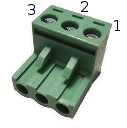
\includegraphics[scale=.3]{figuras/bornera3.png}
	\caption{Bornera de alimentaci\'on.}
	\label{hF_placa_gen_borneras}
\end{figure}

\begin{table}
	\begin{center}
		\begin{tabular}{|c|c|}
			\hline
			Pin & Voltaje \\
			\hline
			1 & GND \\
			\hline
			2 & 5V \\
			\hline
			3 & 7V a 12V \\
			\hline
		\end{tabular}
		\caption{Alimentaci\'on de la l\'ogica}
		\label{hT_placa_gen_alimentacion}
	\end{center}
\end{table}

La regulaci\'on interna de voltaje la realizamos por medio de un regulador 7805 y tiene una corriente m\'axima de 1A.

\paragraph{Configuraci\'on}
\label{h_placas_generica_config}

La fila de pines \emph{P2} exporta todos los pines con funciones dentro del microcontrolador, para realizar
conexiones con perif\'ericos de prueba o nuevas extensiones.
Los headers \emph{P3} y \emph{P4} son jumpers que vinculan los pines \emph{RA1} y \emph{RA4} del
microcontrolador los leds 1 y 2 respectivamente.

El header de programaci\'on \emph{P1} lo utilizamos para conectar la placa con el programador y debuguear
el c\'odigo \emph{ICD2} como explicamos en en apartado \ref{h_controlador_micro_programacion}.
El switch \emph{S2} lo usamos para asociar los pines del microcontrolador con los canales de clock
y data del header de programaci\'on (modo \emph{ICD2}) o con los pines \emph{RB6} y \emph{RB7 }del header
\emph{P2}.

\paragraph{Esquem\'atico}
\label{h_placas_generica_esquematicos}

En la figura \ref{hF_placa_gen_schema1} mostramos el esquem\'atico del microcontrolador y el conexionado
con los headers; el m\'odulo de comunicaci\'on y conectores para conformar la cadena \emph{Daisy-Chain}
los detallamos en la figura \ref{hF_placa_gen_schema2}.
En la figura \ref{hF_placa_gen_schema3} mostramos el diagrama de la fuente de alimentaci\'on y bornera.

\begin{figure}
	\centering
	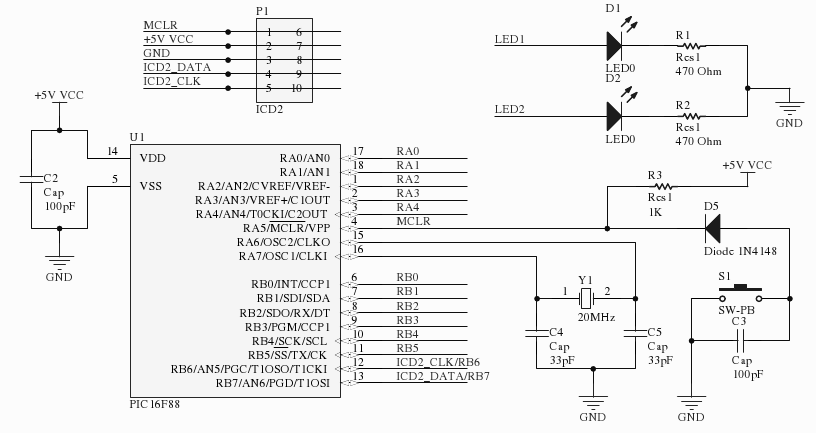
\includegraphics[scale=.32]{figuras/gen_schemaMicro.png}
	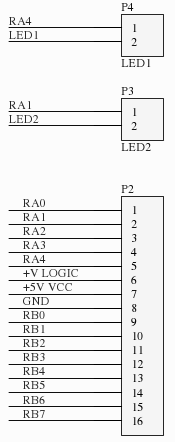
\includegraphics[scale=.32]{figuras/gen_schemaHeaders.png}
	\caption{Microcontrolador y headers}
	\label{hF_placa_gen_schema1}
\end{figure}

\begin{figure}
	\centering
	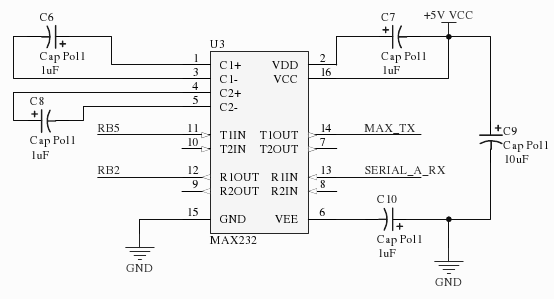
\includegraphics[scale=.3]{figuras/gen_schemaComm1.png}
	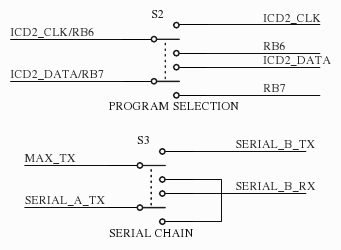
\includegraphics[scale=.3]{figuras/gen_schemaComm2.png}
	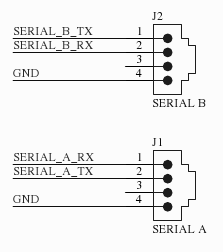
\includegraphics[scale=.3]{figuras/gen_schemaComm3.png}
	\caption{Comunicaci\'on, switch de modo y conectores de entrada y salida}
	\label{hF_placa_gen_schema2}
\end{figure}

\begin{figure}
	\centering
	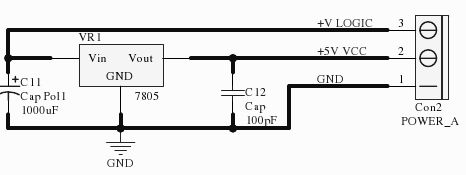
\includegraphics[scale=.3]{figuras/gen_schemaFuente.png}
	\caption{Fuente de alimentaci\'on}
	\label{hF_placa_gen_schema3}
\end{figure}

\paragraph{Circuito}
\label{h_placas_generica_circuito}

En la figura \ref{hF_placa_gen_componentes} mostramos la m\'ascara de componentes de la placa y en
la figura \ref{hF_placa_gen_capas} ambas capas de la placa.

\begin{figure}
	\centering
	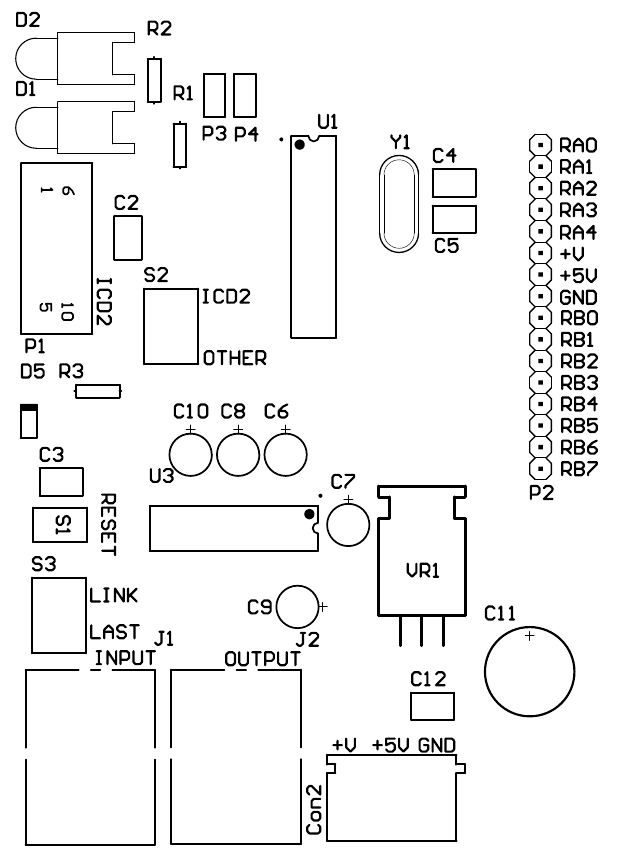
\includegraphics[scale=.2]{figuras/gen_componentes.png}
	\caption{M\'ascara de componentes de la placa gen\'erica.}
	\label{hF_placa_gen_componentes}
\end{figure}

\begin{figure}
	\centering
	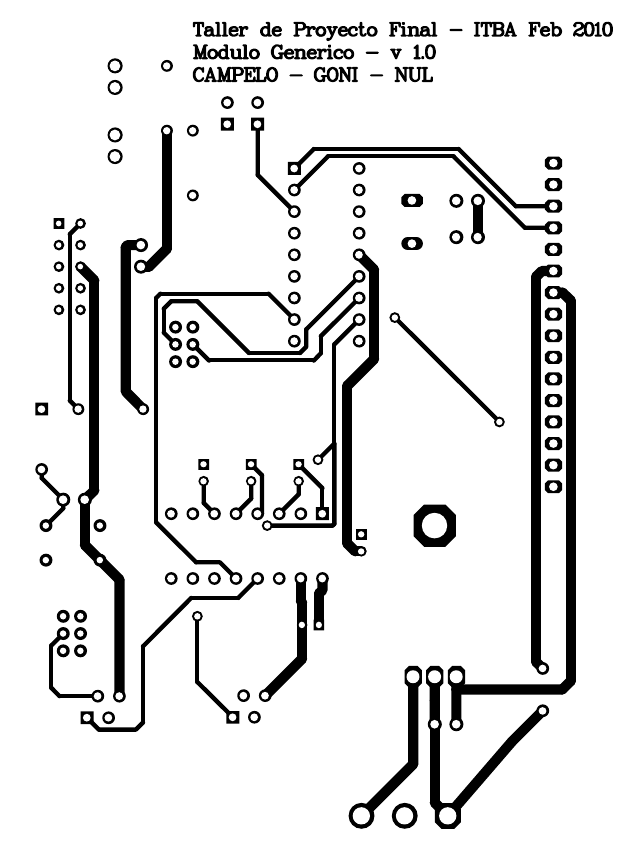
\includegraphics[scale=.2]{figuras/gen_top.png}
	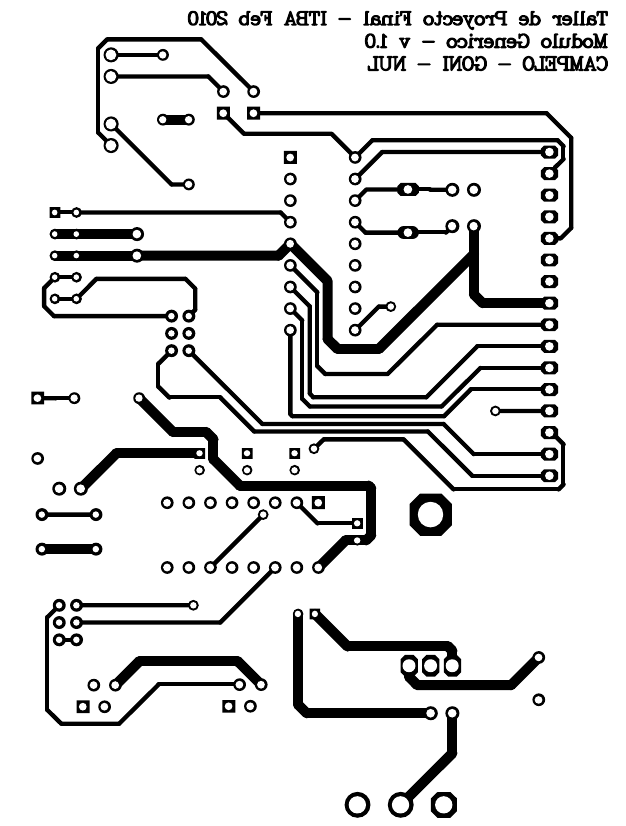
\includegraphics[scale=.2]{figuras/gen_bottom.png}
	\caption{Capas superior e inferior de la placa gen\'erica.}
	\label{hF_placa_gen_capas}
\end{figure}

\paragraph{C\'odigo b\'asico}
\label{h_placas_generica_codigo}

Seg\'un el uso que le fuimos dando a las placas gen\'ericas fuimos cambiando el c\'odigo del firmware que le
\'ibamos cargando, pero siempre manten\'iamos partes b\'asicas que nos ayudaban.

\'Estas principalmente inclu\'ian la configuraci\'on de flags de configuraci\'on base del microcontrolador,
desde la velocidad del clock para los c\'alculos de tiempos hasta determinar que pines eran mapeados a las
funciones de RX y TX para la comunicaci\'on serial.

Para hacer pruebas sobre la comunicaci\'on RS232 o del protocolo, armamos maquetas para las funciones que
atienden a los comandos espec\'ificos y funciones de control del protocolo comunes para todas las placas.
Tambi\'en generamos un modelo general del programa, con un loop principal y llamadas incializadoras.
De esta s\'olo nos concentr\'abamos en la prueba que est\'abamos realizando.

\paragraph{Posibles extensiones}
\label{h_placas_generica_extensiones}

Son varias las extensiones que se podr\'ian realizar a estas placas pero teniendo en cuenta que deb\'ian ser
lo m\'as gen\'ericas posibles como para probar nuevas funcionalidades o componentes, creemos que aportan mucho
valor en la fase de testeo; sin embargo usar componentes de montaje superficial nos hubieran permitido tener
una placa m\'as compacta.

\subsubsection{Placa controladora de motores DC}
\label{h_placas_motorDC}

Nuestro proyecto implicaba, entre otras cosas, el dise\~no y construcci\'on de un robot m\'ovil el cual deb\'ia poder
trasladarse por el terreno como primer requerimiento.
Y debido a que el desplazamiento iba a ser mediante ruedas, el control de los motores que las impulsaran era cr\'itico.

Creamos una placa especializada para esta tarea sobredimensionando los requerimientos para no tener acotadas las opciones
a futuro sobre qu\'e modelo de motores usar\'iamos.

En este apartado explicamos los aspectos que tuvimos en cuenta para dise\~nar y crear la placa controladora de motores
de corriente continua para el robot.

\paragraph{Caracter\'isticas principales}
\label{h_placas_motorDC_caracteristicas}

La funci\'on principal, es entre otras, mantener una velocidad estable en el motor de cont\'inua, pero tambi\'en poder sensar la cantidad
y sentido del movimiento que realiz\'o la rueda, informar el consumo y poder determinar el desplazamiento a realizar.
Este \'ultimo requerimiento era de vital importancia si quer\'iamos tener precisi\'on en el movimiento que realizar\'ia la rueda
ya que este control de r\'apida respuesta hubiera sido imposible hacerlo desde el controlador principal.

Todos los comandos desde y hacia el controlador principal viajan por la red de comunicaci\'on como explicamos en la secci\'on
\ref{h_comm} coloc\'andose como un eslab\'on m\'as en la cadena.
Usamos como base la placa gen\'erica que explicamos en la secci\'on \ref{h_placas_generica} y agregamos el circuito necesario para
el control del motor como explicamos en el punto \ref{h_placas_motorDC_circuito}.

\paragraph{Comunicaci\'on}
\label{h_placas_motorDC_comm}

Al utilizar la placa gen\'erica como base mantuvimos la secci\'on de comunicaci\'on de la misma intacta, pues
en principio, era un m\'odulo probado y funcional, adem\'as manten\'iamos la misma estructura f\'isica que
facilitaba el conexionado para futuros usuarios.

Como explicamos en la secci\'on \ref{h_comm_protocolo_comandosEspecificos} esta placa responde a comandos
espec\'ificos listados en el cuadro \ref{hT_comm_comandos_motordc}.
La principal informaci\'on disponible mediante estos comandos es la velocidad de la rueda en cuentas del
encoder por segundo, el sentido de giro y el hist\'orico de cuentas realizadas.
Podemos enviar comandos para setear estos valores y otros, como la cantidad de cuentas del encoder y a qu\'e
velocidad debe girar la rueda debe hacerlo.

Tambi\'en podemos leer la cantidad de cuentas restantes antes de frenar y el consumo actual del motor para
hacer c\'alculos sobre el tiempo restante de bater\'ia.

\paragraph{Alimentaci\'on de la placa}
\label{h_placas_motorDC_alimentacion}

Como explicamos en la secci\'on \ref{h_placas_generica}, la alimentaci\'on principal de la l\'ogica es
de 7 a 20 volts, con la posibilidad de alimentarla directamente con 5 volts por uno de los pines del conector.
La alimentaci\'on del motor es por una bornera de 2 pines como listamos en el cuadro \ref{hT_placa_dc_alimentacion},
aislada completamente para disminuir as\'i el ruido generado por el funcionamiento del motor sobre la l\'ogica.

\begin{table}
	\begin{center}
		\begin{tabular}{|c|c|}
			\hline
			Pin & Voltaje \\
			\hline
			1 & GND \\
			\hline
			2 & 12v (depende del motor) \\
			\hline
		\end{tabular}
		\caption{Pines de alimentaci\'on del motor.}
		\label{hT_placa_dc_alimentacion}
	\end{center}
\end{table}

Como la alimentaci\'on del motor se hace mediante el \emph{puente H}, no puede superar los $46V$ que es el
m\'aximo que puede operar el \emph{L298}.

Cabe aclarar tambi\'en que al estar ambos circuitos completamente aislados, se necesita unificar ambas masas
para establecer un punto de referencia com\'un y as\'i poder ejercer el control del \emph{puente H} y la lectura
del consumo, de forma correcta.
Recomendamos hacer esto lo m\'as cerca posible de la bater\'ia para disminuir al m\'aximo el ruido que pueda
generarse debido a los motores.

\paragraph{Configuraci\'on}
\label{h_placas_motorDC_config}

La configuraci\'on de la placa es relativamente sencilla.
Antes que nada debemos determinar el rol de la placa dentro de la cadena de comunicaci\'on, esto lo hacemos
mediante el switch \emph{S3}.
Podemos colocarlo en modo \emph{LINK} para que sea un eslab\'on m\'as o en modo \emph{LAST} para que sea
la terminaci\'on de la cadena.

El header del motor comunica la placa con el motor de cont\'inua, en el cuadro \ref{hT_placa_dc_header_motor}
detallamos la posici\'on de los pines.

Las se\~nales \emph{MOTOR\_B} y \emph{MOTOR\_A} son para la alimentaci\'on del motor, dependiendo del sentido
de circulaci\'on de la corriente entre estos pines ser\'a el sentido de giro del motor.
\'Esto se controla desde el puente H \emph{L298}.

Los sensores dentro del motor  reciben tensi\'on mediante los pines \emph{$5V$ VCC} y \emph{GND}.
La se\~nal \emph{IDX} genera pulsos seg\'un las vueltas en el eje de salida de la caja de reducci\'on del
motor.
En cambio las se\~nales \emph{Encoder\_A} o \emph{Encoder\_B} generan pulsos en base a las vueltas del motor
antes de entrar en la caja.

El switch \emph{S2} lo utilizamos para asociar los pines del microcontrolador con el canal de datos del header
de programaci\'on, que explicamos en la secci\'on \ref{h_controlador_micro_programacion}, modo \emph{ICD2} o
con la se\~nal de lectura del encoder.

La se\~nal del encoder proviene a su vez del switch \emph{S4}, el cual nos da la posibilidad de elegir entre
alguna de las dos se\~nales \emph{Encoder\_A} o \emph{Encoder\_B}.

Podemos usar a los pines \emph{P2} y \emph{P3} para tomar como referencia del conversor anal\'ogico digital
a \emph{GND} y \emph{VCC}, o al divisor de tensi\'on formado por las resistencias \emph{R5} y \emph{R6}.

\begin{table}
	\begin{center}
		\begin{tabular}{|c|c|c|c|}
			\hline
			Pin & Se\~nal & Pin & Se\~nal \\
			\hline
			1 & MOTOR\_B & 2 & MOTOR\_A \\
			\hline
			3 & IDX & 4 & - \\
			\hline
			5 & ENCODER\_B & 6 & GND \\
			\hline
			7 & ENCODER\_A & 8 & GND \\
			\hline
			9 & $5V$ VCC & 10 & GND \\
			\hline
		\end{tabular}
		\caption{Pines del header de comunicaci\'on con el motor.}
		\label{hT_placa_dc_header_motor}
	\end{center}
\end{table}

\paragraph{Esquem\'atico}
\label{h_placas_motorDC_esquematico}

En la figura \ref{hF_placa_dc_schema} mostramos el esquem\'atico del microcontrolador y el conexionado el header
de programaci\'on.
En la figura \ref{hF_placa_dc_schema2} detallamos el m\'odulo de comunicaci\'on y el conexionado con los conectores
entre placas.
En la figura \ref{hF_placa_dc_schema3} el esquem\'atico del driver y el header del motor.
En la figura \ref{hF_placa_dc_schema4} mostramos los pines del divisor de tensi\'on para el conversor anal\'ogico
digital y en la figura \ref{hF_placa_dc_schema5} la fuente de alimentaci\'on y borneras.

\begin{figure}
	\centering
	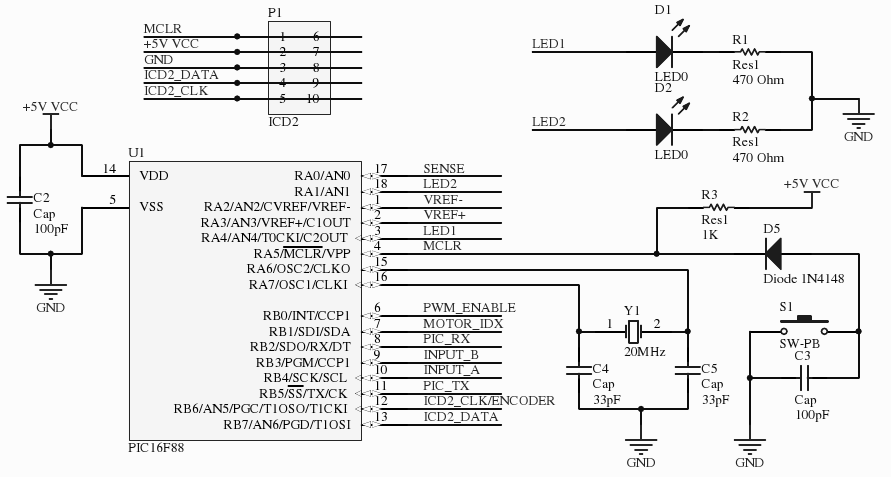
\includegraphics[scale=.3]{figuras/dc_schemaMicro.png}
	\caption{Microcontrolador y header de programaci\'on.}
	\label{hF_placa_dc_schema}
\end{figure}

\begin{figure}
	\centering
	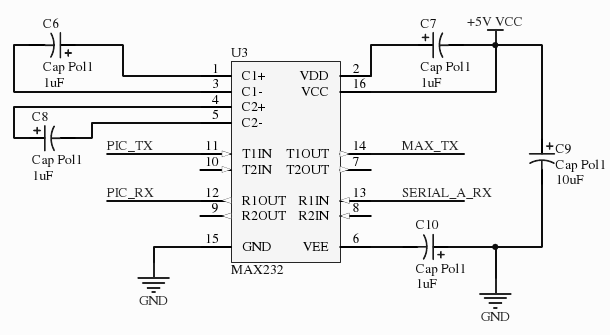
\includegraphics[scale=.28]{figuras/dc_schemaComm1.png}
	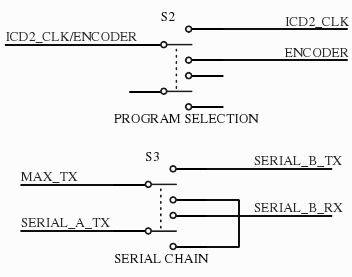
\includegraphics[scale=.28]{figuras/dc_schemaComm2.png}
	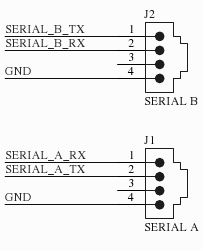
\includegraphics[scale=.28]{figuras/dc_schemaComm3.png}
	\caption{Comunicaci\'on, switch de modo y conectores de entrada y salida.}
	\label{hF_placa_dc_schema2}
\end{figure}

\begin{figure}
	\centering
	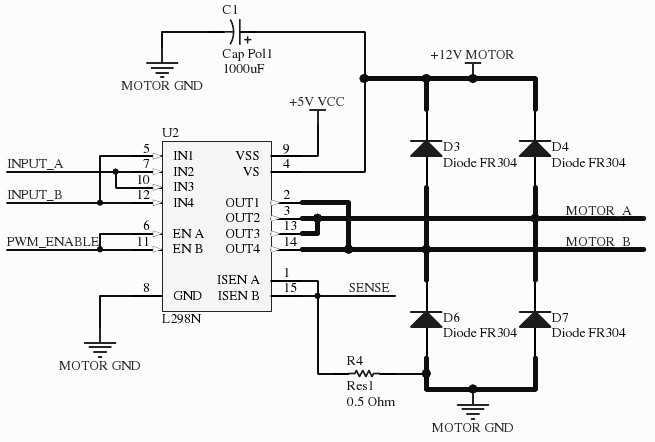
\includegraphics[scale=.3]{figuras/dc_schemaDriver.png}
	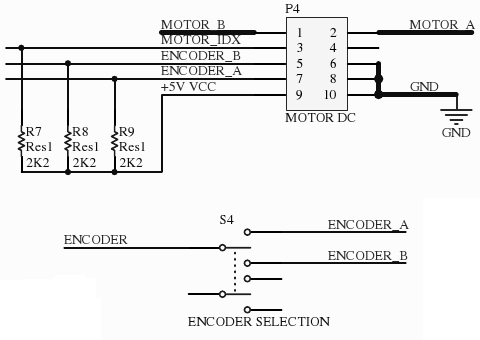
\includegraphics[scale=.3]{figuras/dc_schemaMotorEncoder.png}
	\caption{Driver y header de conexi\'on con el motor.}
	\label{hF_placa_dc_schema3}
\end{figure}

\begin{figure}
	\centering
	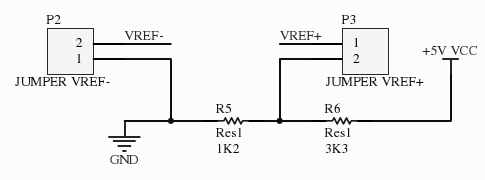
\includegraphics[scale=.3]{figuras/dc_schemaADC.png}
	\caption{Divisor de tensi\'on para el voltaje de referencia.}
	\label{hF_placa_dc_schema4}
\end{figure}

\begin{figure}
	\centering
	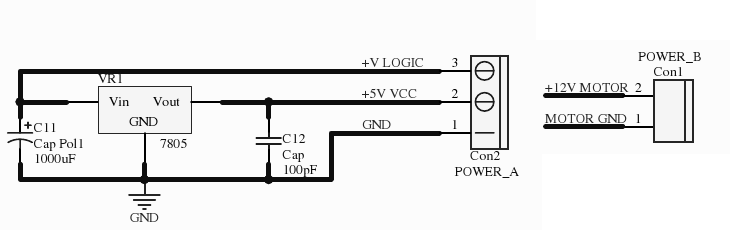
\includegraphics[scale=.3]{figuras/dc_schemaFuente.png}
	\caption{Fuente de alimentaci\'on de la l\'ogica y motor.}
	\label{hF_placa_dc_schema5}
\end{figure}

\paragraph{Circuito}
\label{h_placas_motorDC_circuito}

En la figura \ref{hF_placa_dc_componentes} mostramos la m\'ascara de componentes de la placa.
En la figura \ref{hF_placa_dc_capas} mostramos ambas capas de la placa.

\begin{figure}
	\centering
	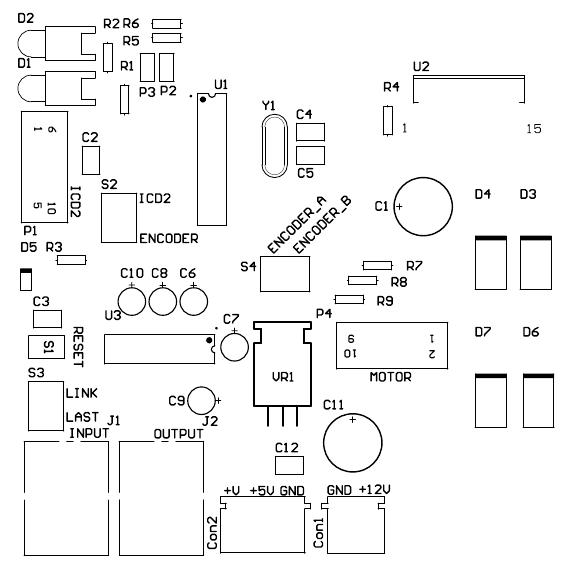
\includegraphics[scale=.3]{figuras/dc_componentes.png}
	\caption{M\'ascara de componentes de la placa controladora de motores DC.}
	\label{hF_placa_dc_componentes}
\end{figure}

\begin{figure}
\centering
	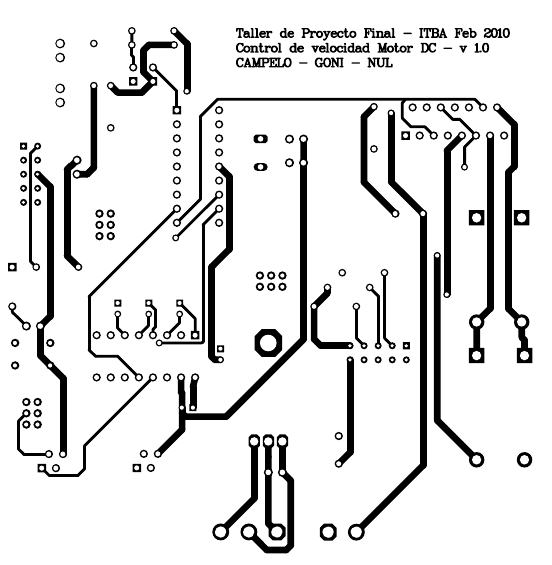
\includegraphics[scale=.3]{figuras/dc_top.png}
	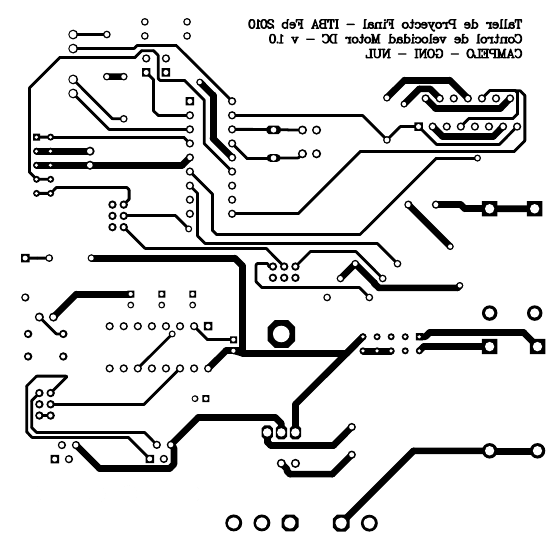
\includegraphics[scale=.3]{figuras/dc_bottom.png}
	\caption{Capas superior e inferior de la placa controladora de motores DC.}
	\label{hF_placa_dc_capas}
\end{figure}

\paragraph{C\'odigo b\'asico}
\label{h_placas_motorDC_codigo}

El c\'odigo m\'inimo para ser parte de la cadena de comunicaci\'on es similar al de todas las placas que
armamos.
La personalizaci\'on del c\'odigo est\'a dentro de la funci\'on que interpreta el comando recibido y realiza
las tareas internas necesarias para llevar a cabo dicha acci\'on y depende \'integramente del protocolo.

Para el sensado de la velocidad debemos determinar cu\'ales son los pines de lectura de la se\~nal del encoder
y debemos generar una base de tiempo que nos permita establecer cu\'antas cuentas del encoder hay por intervalo
de tiempo.
Con dicha informaci\'on podemos aumentar o disminuir el ancho del pulso que controla al puente H \emph{L298}
y, en consecuencia, controlar la velocidad del motor de corriente cont\'inua.

Para mantener un hist\'orico de cuentas de encoder realidas nosotros usamos el conocimiento del sentido de giro
del motor para sumar o restar el valor calculado por cada intervalo de tiempo en una variable interna del
microcontrolador.

\paragraph{Posibles extensiones}
\label{h_placas_motorDC_extensiones}

Un punto recurrente de discusi\'on fue el uso de una placa por cada motor de corriente cont\'inua.
Sab\'iamos que era posible realizar todas las funciones necesarias para el control de dos motores en una \'unica
placa, pero esto nos tra\'ia una mayor complejidad tanto a nivel f\'isico como a nivel l\'ogico de control, y un
tiempo de implementaci\'on superior.
Es por estas razones que decidimos esta configuraci\'on y dejarlo como futura extensi\'on para la cual usar\'iamos
los conocimientos y experiencias adquiridas en el desarrollo de la actual.

Otra posible extensi\'on que es recurrente en todas las placas es el uso de componentes de montaje superficial
lo que disminuir\'ia el tama\~no de la misma en gran medida pero a su vez implicaba cierta complejidad que preferimos
evitar en el desarrollo del prototipo.

\subsubsection{Placas de sensado}
\label{h_placas_sensado}

Para sensar el entorno utilizamos distintos tipos de sensores que deb\'iamos leer y controlar seg\'un fuera
requerido desde el controlador principal.
Dise\~namos una placa a la que podemos conectarle cualquiera de los sensores que usamos en nuestro proyecto,
ya sea un sensor de distancia por ultrasonido, tel\'emetros o sensores reflectivos de piso.
Tamb\'ien utilizamos esta placa para realizar las lecturas de la tensi\'on de la bater\'ia.
En este apartado detallamos cada una de las caracter\'isticas que tuvimos en cuenta durante el desarrollo
de las placas de sensado.

\paragraph{Caracter\'isticas principales}
\label{h_placas_sensado_caracteristicas}

El uso de diferentes tipos de sensores implicaba un m\'etodo distinto de lectura seg\'un qu\'e sensor
estaba conectado.
Los sensores de distancia por ultrasonido que usamos generan un pulso de ancho variable seg\'un la
distancia al objetivo.
De forma similar, los tel\'emetros setean un voltaje en la salida en base a la
distancia con el objeto.
Los sensores reflectivos de piso que usamos miden el nivel de luz infrarroja que refleja la superficie
que tienen debajo de ellos y en base al valor sensado inferimos su color.

Para los sensores que devuelven el valor sensado mediante un voltaje, utilizamos el conversor anal\'ogico
digital para tomar las muestras necesarias.
Salvo que se indique lo contrario, tomamos $5$ muestras y luego las promediamos para minimizar el error
de muestreo.

En el caso del sensor de ultrasonido usamos el m\'odulo de timer para calcular el ancho del pulso
generado por el sensor.
Tambi\'en usamos interrupciones para captar los flancos ascendentes y descendentes para determinar el
comienzo y fin del pulso respectivamente.

Armamos la placa para poder conectar un sensor de distancia por ultrasonido o un switch binario sobre
el mismo puerto de conexi\'on.
De manera conjunta podemos conectar a la misma placa, hasta cinco sensores por voltaje, tel\'emetros,
fototransistores (sensores de piso) o por ejemplo el divisor de tensi\'on que mide la carga en la bater\'ia.

Generamos la posibilidad de habilitar y deshabilitar la alimentaci\'on de estos sensores mediante el uso
de un transistor \emph{BC327} y as\'i aumentar la autonom\'ia del robot.
Este transistor tiene una corriente m\'axima de hasta $500mA$ para alimentar al sensor que sea necesario.

\paragraph{M\'odulo de comunicaci\'on}
\label{h_placas_sensado_comm}

De igual forma que las otras placas en el proyecto, mantenemos la misma disposici\'on f\'isica de
la comunicaci\'on, desde el circuito base hasta la ubicaci\'on de los conectores para mayor facilidad
a la hora de utilizarlas.
Tambi\'en respetamos el protocolo de comunicaci\'on definiendo nuevos comandos espec\'ificos para la
placa y retransmitiendo los paquetes con otro destinatario.

\paragraph{Alimentaci\'on de la placa}
\label{h_placas_sensado_alimentacion}

De igual forma que las otras placas la alimentaci\'on principal de la l\'ogica es de 7 a 20 volts,
con la posibilidad de alimentarla directamente con 5 volts por uno de los pines del conector como
explicamos en la secci\'on \ref{h_placas_generica}.

\paragraph{Configuraci\'on}
\label{h_placas_sensado_config}

Para la configuraci\'on f\'isica de la placa necesitamos definir primero el rol de la placa dentro de
la cadena de comunicaci\'on con la llave \emph{S3}.
Como en todas las placas que dise\~namos s\'olo tenemos que elegir el modo \emph{LAST} o \emph{LINK}
para determinar si es la terminaci\'on o un eslab\'on m\'as en la cadena.

Debemos saber que no podemos conectar m\'as de $5$ sensores de los cuales debamos medir una tensi\'on
para obtener el valor.
S\'olo un sensor de distancia por ultrasonido o switch en el puerto para
medir estados l\'ogicos y tiempo del pulso.

Con la llave \emph{S2} cambiamos al modo programaci\'on vinculando el microcontrolador con el header
de \emph{ICD2} o con la habilitaci\'on de los puertos de los sensores \emph{3} y \emph{4}.
Si esta llave esta en la posici\'on incorrecta nunca se exitar\'a el transistor y por ende no habr\'a
alimentaci\'on en el sensor.

En el caso que necesitemos una resistencia \emph{pull-up} conectada con la salida del sensor podemos
colocar un jumper en el correspondiente header de pull-up del puerto de sensor.

\paragraph{Esquem\'atico}
\label{h_placas_sensado_esquematico}

En la figura \ref{hF_placa_sense_schema} mostramos el esquem\'atico del microcontrolador y el conexionado
del header de programaci\'on.
En la figura \ref{hF_placa_sense_schema2} detallamos el m\'odulo de comunicaci\'on y el conexionado con
los conectores entre placas.

En la figura \ref{hF_placa_sense_schema3} mostramos los puertos de conexi\'on para cada uno de los sensores
y en la figura \ref{hF_placa_sense_schema4} la fuente de alimentaci\'on y bornera.

\begin{figure}
	\centering
	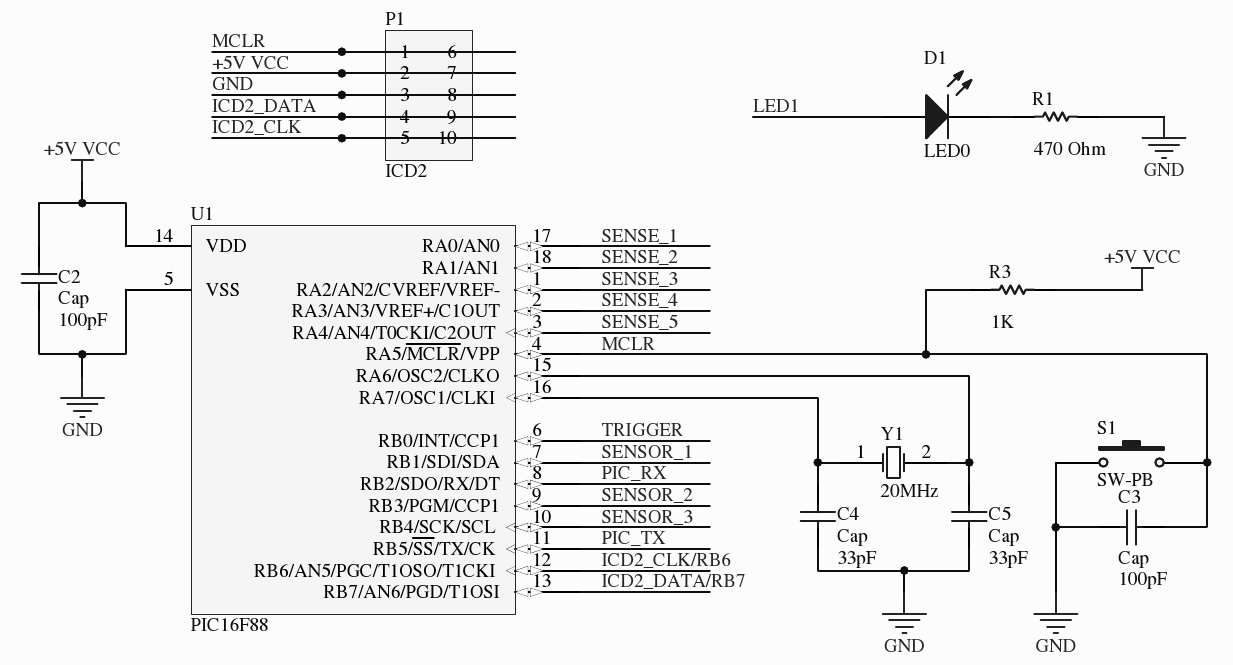
\includegraphics[scale=.22]{figuras/sense_schemaMicro.png}
	\caption{Microcontrolador y header de programaci\'on.}
	\label{hF_placa_sense_schema}
\end{figure}

\begin{figure}
	\centering
	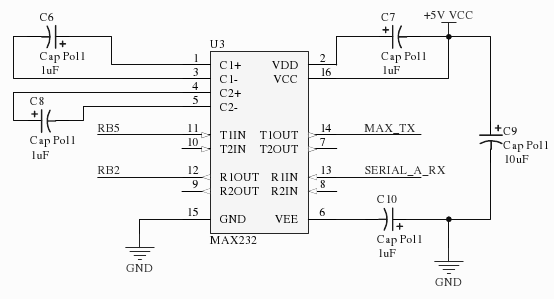
\includegraphics[scale=.28]{figuras/sense_schemaComm1.png}
	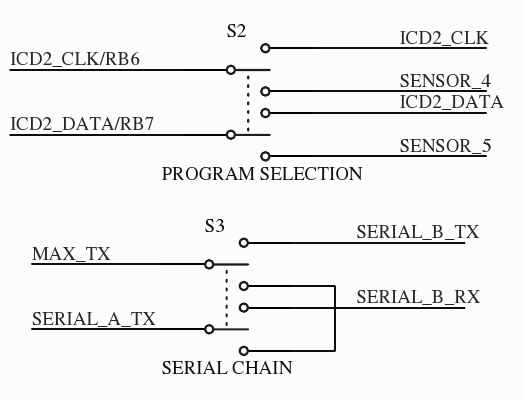
\includegraphics[scale=.2]{figuras/sense_schemaComm2.png}
	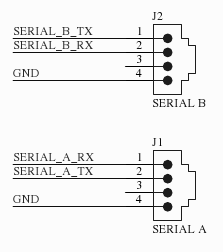
\includegraphics[scale=.28]{figuras/sense_schemaComm3.png}
	\caption{Comunicaci\'on, llaves de modo y conectores de entrada y salida.}
	\label{hF_placa_sense_schema2}
\end{figure}

\begin{figure}
	\centering
	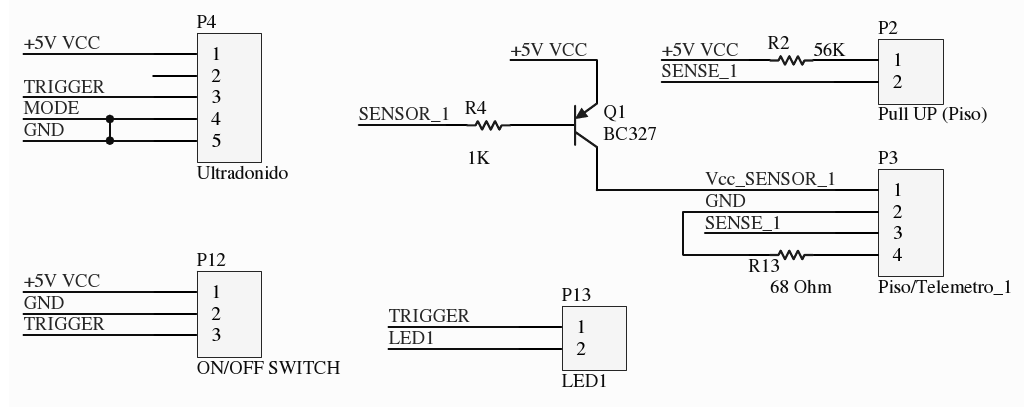
\includegraphics[scale=.28]{figuras/sense_schemaSensor.png}
	\caption{Puertos de conexi\'on para los sensores y header de \emph{pull-up}.}
	\label{hF_placa_sense_schema3}
\end{figure}

\begin{figure}
	\centering
	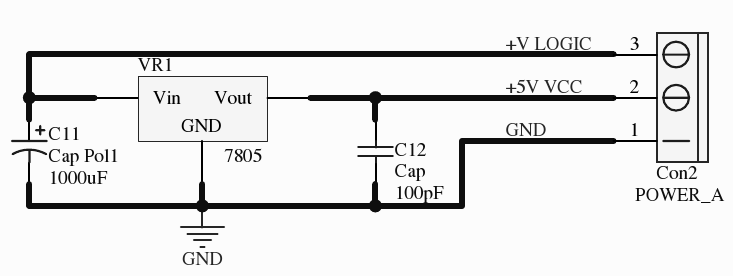
\includegraphics[scale=.22]{figuras/sense_schemaFuente.png}
	\caption{Fuente de alimentaci\'on de la l\'ogica.}
	\label{hF_placa_sense_schema4}
\end{figure}

\paragraph{Circuito}
\label{h_placas_sensado_circuito}

En la figura \ref{hF_placa_sense_componentes} mostramos la m\'ascara de componentes de la placa.
En la figura \ref{hF_placa_sense_capas} mostramos ambas capas de la placa.

Una observaci\'on importante en el circuito de esta placa es que al momento de montarla
observamos una gran inestabilidad en el microcontrolador cuando hac\'iamos lecturas simult\'aneas
en m\'as de 2 tel\'emetros.
Luego de varios intentos para solucionar este inconveniente, descubrimos que era un problema
en cuanto a un consumo instant\'aneo de los tel\'emetros que generaba que se reseteara el
microcontrolador.
Para solucionar esto colocamos un capacitor de $100\mu F$ entre las pistas de \emph{+5V} y
\emph{GND} en medio de los puertos de los sensores 1 y 2.

Luego de este peque\~no cambio pudimos seguir con nuestro desarrollo y las siguiente pruebas
mostraron la estabilidad que necesitabamos en el microcontrolador.

\begin{figure}
	\centering
	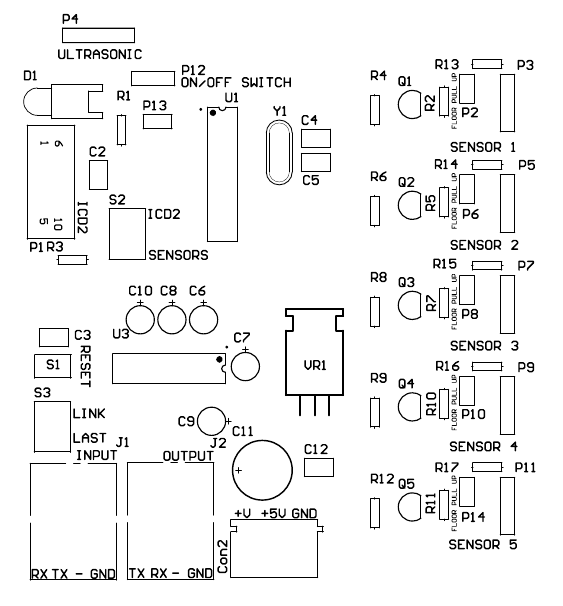
\includegraphics[scale=.3]{figuras/sense_componentes.png}
	\caption{M\'ascara de componentes de la placa controladora de sensores.}
	\label{hF_placa_sense_componentes}
\end{figure}

\begin{figure}
\centering
	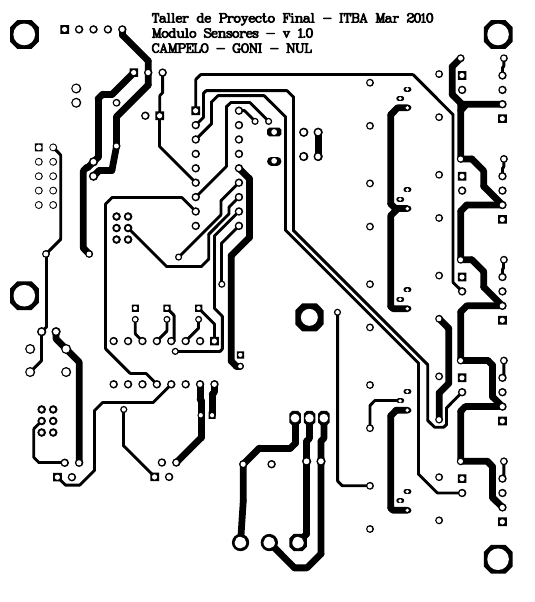
\includegraphics[scale=.3]{figuras/sense_top.png}
	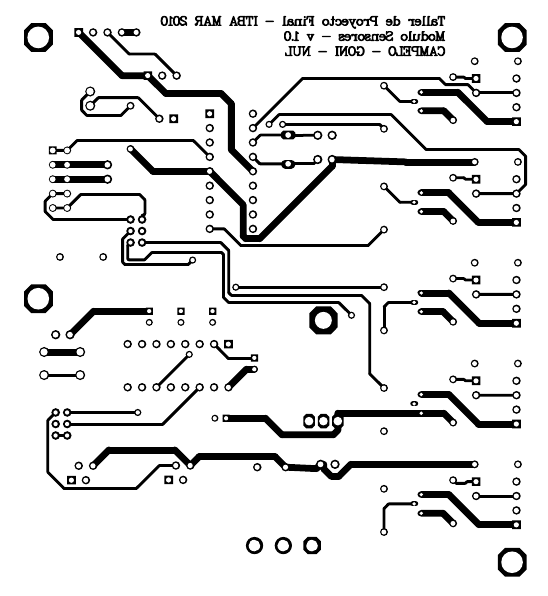
\includegraphics[scale=.3]{figuras/sense_bottom.png}
	\caption{Capas superior e inferior de la placa controladora de sensores.}
	\label{hF_placa_sense_capas}
\end{figure}

\paragraph{C\'odigo b\'asico}
\label{h_placas_sensado_codigo}

Al compartir el m\'odulo de comunicaci\'on entre las placas y para que nuestra placa sea parte de la
cadena y podamos interpretar los paquetes que viajan por ella, debemos incluir el c\'odigo com\'un
de comunicaci\'on e implementar la funci\'on que analiza y ejecuta los paquetes que son dirigidos
directamente a nuestra placa, grupo o a nivel broadcast.

Dependiendo de la selecci\'on de los sensores a conectar ser\'a la configuraci\'on interna del microcontrolador.
Al principio del c\'odigo colocamos una serie de scripts que nos ayudan a configurar los tiempos a los que se
deben tomar las muestras de los sensores y los flags del microcontrolador.

Los pines que exitan a la base de los transistores usan una l\'ogica inversa, es decir, un estado bajo habilita
la alimentaci\'on del sensor y un estado alto, lo deshabilita.

\paragraph{Posibles extensiones}
\label{h_placas_sensado_extensiones}

Dentro de las posibles extensiones que creemos que ser\'ian \'utiles a futuro podemos decir que la m\'as
significativa ser\'ia usar potenci\'ometros en vez de resistencias fijas para usar como \emph{pull-up} y
para variar la alimentaci\'on de los sensores de piso por ejemplo.

En una implementaci\'on futura tambi\'en agregar\'iamos el uso de componentes de montaje superficial y
aumentar\'iamos la cantidad de puertos para sensores disponibles.
De igual forma, incorporar otro tipo de sensores nos parece una interesante mejora.

\subsubsection{Placa controladora de servo motores}
\label{h_placas_servos}

Para los mecanismos que implicaban alg\'un tipo de movimiento y control de la posici\'on elegimos usar
de servo motores, ya sea para el mecanismo de recolecci\'on de basura, inclinar el robot, reclinar el
cesto interno de basura o realizar alg\'un movimiento de paneo o foco con la c\'amara.

Dise\~namos esta placa teniendo en cuenta que usar\'iamos varios servos en el robot y que tambi\'en
necesitar\'iamos tener la posibilidad de recibir se\~nales del estilo \emph{fin de carrera} o alg\'un
est\'imulo generado por pulsadores que modificaran o no el accionar de los motores.

Esta placa no la construimos para este prototipo debido a que no cont\'abamos con la necesidad.
Al no implementar ning\'un m\'etodo f\'isico de recolecci\'on, no ten\'iamos mecanismos que la
usaran, aunque s\'i entendimos que era algo que deb\'iamos hacer para tener el conocimiento y sentar
una base para futuras implementaciones o proyectos similares.

\paragraph{Caracter\'isticas principales}
\label{h_placas_servos_caracteristicas}

Dise\~namos la placa pensando en que tendr\'iamos que controlar cinco servo motores.
Debido a que pensamos usar servo motores de tipo digital necesit\'abamos varios m\'odulos de PWM para
realizar esta tarea.
Pensamos en el uso de otros microcontroladores que pudieran proveernos de esta facilidad, pero finalmente
decidimos implementar esta funcionalidad por software.

A los puertos que no estan destinados al control de los servo motores les podemos dar varios usos.
En un principio los pensamos como generadores interrupciones ante un cambio en el estado y en el
puerto \emph{P9} contamos con la posibilidad de determinar el flanco ante el cual se generar\'a la
interrupci\'on.
En el puerto \emph{P8} podemos colocar alg\'un tipo de sensado que haga uso del conversor anal\'ogico
digital del microcontrolador.

De igual forma podr\'iamos extender la rutina que genera el PWM por software, a todos los puertos y
controlar hasta $11$ servos con una \'unica placa.

\paragraph{M\'odulo de comunicaci\'on}
\label{h_placas_servos_comm}

Como utilizamos como base las otras placas y mantuvimos la secci\'on de comunicaci\'on, para ser parte
de la cadena s\'olo debemos incluir el c\'odigo com\'un e implementar las acciones necesarias dentro
de la funci\'on que interpreta los comandos a los que somos destinatarios.

Como explicamos en la secci\'on \ref{h_comm_protocolo_comandosEspecificos} creamos ciertos comandos
o paquetes espec\'ificos para el control de los servos.
De igual forma contemplamos el uso de pulsadores en la misma.

Un mayor cambio a nivel funcional implicar\'ia que hicieramos otros cambios a nivel protocolo, el cual
pensamos para ser expandido creando nuevos comandos o modificando los existentes.

\paragraph{Alimentaci\'on de la placa}
\label{h_placas_servos_alimentacion}

Al igual que las otras placas utilizamos entre 7 y 20 volts para alimentar la placa, con la posibilidad
de entregar $5$ volts en forma directa usando el pin indicado.

Hicimos una modificaci\'on importante para la alimentaci\'on en esta placa que nos permitir\'ia entregar
una mayor cantidad de corriente que los $500 mA$ que soporta el integrado \emph{7805} usando transistores
de potencia como los \emph{TIP42}.
Este cambio era importante porque los servo motores que \'ibamos a usar se alimentaban directamente a $5V$
y el consumo en conjunto superaba la cantidad de corriente que el regulador de tensi\'on entregaba.

\paragraph{Configuraci\'on}
\label{h_placas_servos_config}

La configuraci\'on f\'isica necesaria en la placa ser\'ia m\'inima.
Mediante la llave inversora \emph{S2} tendr\'iamos la posibilidad de conectar el microcontrolador
con el header de programaci\'on o puertos \emph{P12} y \emph{P13}.

Usando la llave \emph{S3} establecer\'iamos la posici\'on de la placa dentro de la cadena, ya sea
como la terminaci\'on o un eslab\'on m\'as.
Todas las dem\'as configuraciones ser\'ian a nivel software.

\paragraph{Esquem\'atico}
\label{h_placas_servos_esquematico}

En la figura \ref{hF_placa_servo_schema} mostramos el esquem\'atico del microcontrolador y el conexionado
del header de programaci\'on.
En la figura \ref{hF_placa_servo_schema2} detallamos el m\'odulo de comunicaci\'on y el conexionado con
los conectores entre placas.

En la figura \ref{hF_placa_servo_schema3} mostramos los puertos de conexi\'on para los servo motores y de
uso general para otras conexiones.
En la figura \ref{hF_placa_servo_schema4} la fuente de alimentaci\'on y bornera.

\begin{figure}
	\centering
	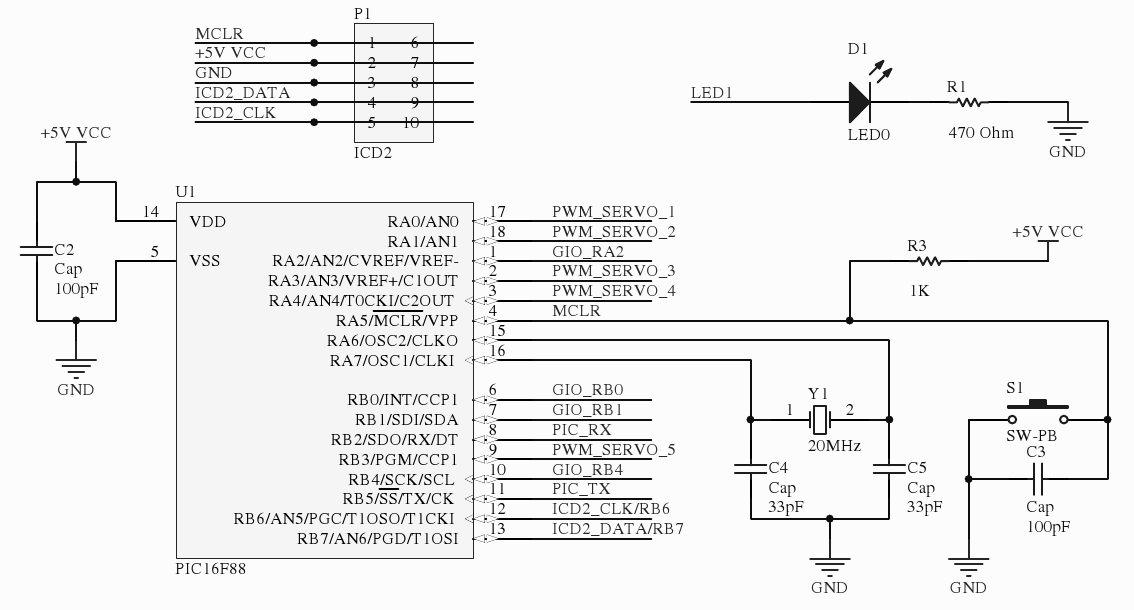
\includegraphics[scale=.22]{figuras/servo_schemaMicro.png}
	\caption{Microcontrolador y header de programaci\'on.}
	\label{hF_placa_servo_schema}
\end{figure}

\begin{figure}
	\centering
	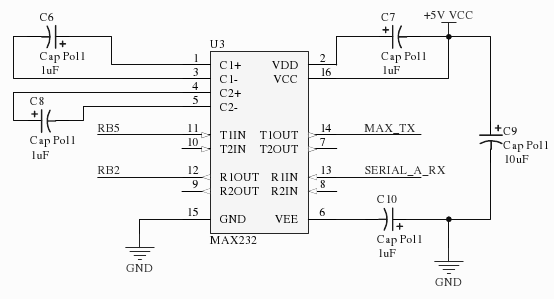
\includegraphics[scale=.28]{figuras/servo_schemaComm1.png}
	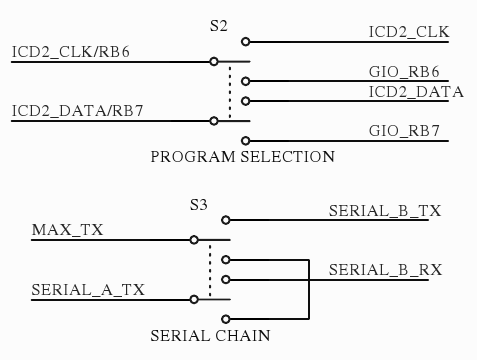
\includegraphics[scale=.2]{figuras/servo_schemaComm2.png}
	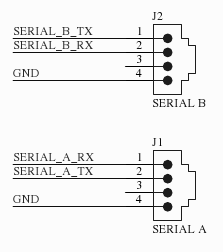
\includegraphics[scale=.28]{figuras/servo_schemaComm3.png}
	\caption{Comunicaci\'on, llaves de modo y conectores de entrada y salida.}
	\label{hF_placa_servo_schema2}
\end{figure}

\begin{figure}
	\centering
	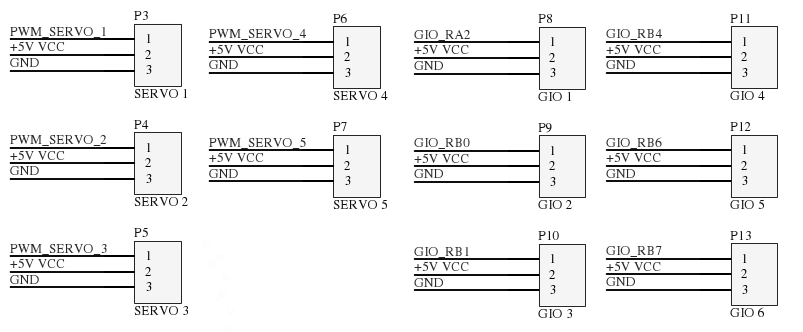
\includegraphics[scale=.35]{figuras/servo_schemaPort.png}
	\caption{Puertos de conexi\'on para los servo motores y de uso general.}
	\label{hF_placa_servo_schema3}
\end{figure}

\begin{figure}
	\centering
	\includegraphics[scale=.3]{figuras/servo_schemaFuente.png}
	\caption{Fuente de alimentaci\'on extendida para la l\'ogica y servo motores.}
	\label{hF_placa_servo_schema4}
\end{figure}

\paragraph{Circuito}
\label{h_placas_servos_circuito}

En la figura \ref{hF_placa_servo_componentes} mostramos la m\'ascara de componentes de la placa.
En la figura \ref{hF_placa_servo_capas} mostramos ambas capas de la placa.

\begin{figure}
	\centering
	\includegraphics[scale=.33]{figuras/servo_componentes.png}
	\caption{M\'ascara de componentes de la placa controladora de servo motores.}
	\label{hF_placa_servo_componentes}
\end{figure}

\begin{figure}
	\centering
	\includegraphics[scale=.3]{figuras/servo_top.png}
	\includegraphics[scale=.3]{figuras/servo_bottom.png}
	\caption{Capas superior e inferior de la placa controladora de servo motores.}
	\label{hF_placa_servo_capas}
\end{figure}

\paragraph{C\'odigo b\'asico}
\label{h_placas_servos_codigo}

Como explicamos en la secci\'on \ref{h_actuadores_servo_rutinas} creamos una rutina de control
que usando el timer del microcontrolador como base de tiempo, genera pulsos del ancho necesario
en cada puerto para establecer la posici\'on necesaria de cada servo motor.

Para capturar cambios de estado en los puertos de uso generar s\'olo deber\'iamos configurar las
interrupciones del microcontrolador para que se generen ante cualquier cambio y verificar en la
rutina de interrupci\'on, que puerto la gener\'o.

De querer utilizar los puertos para funciones no previstas en nuestro dise\~no deber\'iamos
agregar las funciones de control en el ciclo principal de nuestro c\'odigo.

\paragraph{Posibles extensiones}
\label{h_placas_servos_extensiones}

Posiblemente haya necesidades que no contemplamos en es dise\~no de esta placa aunque por no
haberla construido no tenemos la experiencia sobre qu\'e cosas hubi\'eramos hecho diferente.

\subsection{Armado del prototipo}
\label{h_prototipo}

Una vez dise\~nadas, armadas y probadas cada una de las placas controladoras tanto en forma separada
como en conjunto, procedimos al armado del robot prototipo.
Como no ten\'iamos las dimensiones o requerimientos de espacio del mecanismo de recolecci\'on
armamos el prototipo sin estas consideraciones.

\subsubsection{Dise\~no}
\label{h_prototipo_disenio}

Para darle forma al prototipo tuvimos en consideraci\'on varias cuestiones como
\begin{inparaenum}[\itshape a\upshape)]
\item materiales de contrucci\'on;
\item volumen interior para alojar los distintos componentes;
\item posici\'on de cada sensor respecto del borde exterior;
\item posici\'on de las ruedas y la maniobrabilidad que tendr\'ia;
\item deb\'ia poder pasar por entre las sillas y mesas de la terraza.
\end{inparaenum}

Elegimos darle al chasis una forma de oct\'ogono.
\'Esto eliminaba los \'angulos rectos de los bordes para minimizar la posibilidad de quedar
atascados en las esquinas.
A su vez, si coloc\'abamos las ruedas alineadas con el centro geom\'etrico del robot aumentaba la
maniobrabilidad y pod\'iamos realizar r\'apidas rotaciones sin chocar con el entorno.

Respetando nuestro dise\~no inicial y sabiendo que la cantidad de sensores era adecuada para cubrir
nuestros requerimientos, definimos las posiciones de cada sensor.
Para colocar los tel\'emetros infrarrojos a la altura necesaria creamos un contorno con paredes,
que a su vez, nos daban el volumen interior para alojar las placas controladoras y bater\'a.
El sensor de distancia por ultrasonido lo colocamos al frente, centrado y apuntando hacia adelante
para tener el mayor campo de visi\'on posible.

Para sostener las placas en el interior colocamos una varilla roscada de lado a lado en el interior
y afirmamos entre dos tuercas a cada placa.
Colocamos las placas de sensado en el centro y contra las paredes a las placas controladoras de motor.
El cableado con los sensores lo hicimos interior a traves de agujeros en las paredes.
De igual forma, los cables de control para los motores y el cableado para los sensores de piso, los
pasamos por un agujero en la base del robot.

Elegimos una beter\'ia de gel de 12V 7Ah que seg\'un nuestros c\'alculos nos dar\'ia una autonom\'ia
de entre 2 y 3 horas de uso cont\'inuo.
Aprovechando su peso la colocamos lo m\'as atras posible dentro del volumen interior para mover
el centro de gravedad y en conjunto con la rueda castor trasera, dar mayor estabilidad al robot.

Colocamos los motores en la parte inferior del robot alineados con el centro geom\'etrico y las
ruedas dentro del chasis para evitar atascos.
Las ruedas que elegimos tienen una buje de tefl\'on, con llanta de chapa y cubierta de goma compacta.
Un problema que encontramos en este punto fue que el eje del motor era cil\'indrico y no presentaba
ninguna marca o corte para ajustar las ruedas.
Debido a \'esto nos fue muy dif\'icil realizar este ajuste.

Con las ruedas actuales de $10cm$ de di\'ametro y teniendo en cuenta que el motor gira aproximadamente
a $300$ cuentas por segundo, logramos una velocidad cercana a $50 cm/s$.

En la parte superior armamos, con una madera m\'as fina, un segundo piso para cololar la netbook y poder
controlarla f\'acilmente.
Pasamos el cable adaptador USB a serial RS232 por un agujero en el segundo piso y colocamos a la vista
un interruptor de encendido desde el cual podemos recargar la bater\'ia del robot con los cables con
punta de cocodrilo del cargador autom\'atico.

\subsubsection{Desarme}
\label{h_prototipo_desarme}

Para lograr el desarme del prototipo recomendamos desconectar el cable del conversor USB - RS232 y
retirarde la parte superior la netbook.
Luego seguir los siguientes pasos seg\'un las referencias en las figuras \ref{hF_desarme_1}, \ref{hF_desarme_2} y \ref{hF_desarme_3}.

\begin{itemize}
 \item Retirar los $12$ tornillos (1) que sostienen la tapa superior.
 \item Retirar el cable que conecta el sensor de ultrasonido (2) con las placas.
 \item Aflojar los tornillos (3) que sostienen al sensor de ultrasonido.
 \item Retirar la tapa (4).
 \item Desconectar los cables (5) de alimentaci\'on de las placas.
 \item Desconectar los cables (6) que conectan a los tel\'emetros con las placas.
 \item Desconectar los cables (7) de comunicaci\'on entre las placas.
 \item Desconectar los cables (8) que conectan a las placas con los motores DC.
 \item Aflojar y retirar las tuercas (9) que mantienen a la varilla roscada (10).
 \item Despegar y retirar la bater\'ia (11) de la base del robot (12).
 \item Moviendo la varilla hacia los costados, retirar las placas (13).
 \item Retirar los tel\'emetros (14).
 \item Retirar los sensores de piso (15).
 \item Aflojar y retirar las tuercas (16) que sostienen a los sensores de piso.
 \item Retirar las ruedas (17) de los motores.
 \item Retirar los tornillos (18) de las abrazaderas (19) de los motores (20).
 \item Retirar la rueda de tipo castor trasera (21).
 \item Retirar la rueda de tipo castor delantera (22).
\end{itemize}

\begin{figure}
	\centering
	\includegraphics[scale=.45]{figuras/desarme_e.png}
	\caption{Diagrama de desarme exterior.}
	\label{hF_desarme_1}
\end{figure}

\begin{figure}
	\centering
	\includegraphics[scale=.45]{figuras/desarme_f.png}
	\caption{Diagrama de desarme frontal.}
	\label{hF_desarme_2}
\end{figure}

\begin{figure}
	\centering
	\includegraphics[scale=.45]{figuras/desarme_i.png}
	\caption{Diagrama de desarme interior.}
	\label{hF_desarme_3}
\end{figure}

